%-------------------------------- Configurações --------------------------------

\documentclass[a4paper, abntfigtabnum, noindentfirst, normaltoc, pnumplain, notimes]{abnt}

\newcommand{\bc}{NavyBlue}

\usepackage[Sonny]{fncychap}

\usepackage{subfigure}

\usepackage[utf8]{inputenc} % para pode escrever caracteres acentuados normalmente
\usepackage[brazil]{babel}
\usepackage{graphicx}
\usepackage[usenames,dvipsnames]{xcolor} % http://en.wikibooks.org/wiki/LaTeX/Colors
\usepackage[pdfborder={0 0 0},pdfborderstyle={/S/U/W 0.5},citebordercolor=\bc,filebordercolor=\bc,urlbordercolor=\bc,linkbordercolor=\bc]{hyperref} % http://www.tug.org/applications/hyperref/manual.html e http://migre.me/7FH3e
\usepackage[alf]{abntcite}
\usepackage{booktabs} % para utilização das linhas separadoras na tabela
\usepackage{textcomp}
%\usepackage{minted} % foi adicionado o seguinte hack no minted: http://migre.me/7M8wI
\usepackage{nomencl} % para criar a lista de siglas

\usepackage{amsmath}

%----------------------- Números de Figuras e Tabelas no Formato Capítulo.número_da_Figura ------------------------

\newcommand{\Chapter}[1]{\chapter{#1} \setcounter{figure}{0} \setcounter{table}{0}}
\renewcommand{\thefigure}{\arabic{chapter}.\arabic{figure}}
\renewcommand{\thetable}{\arabic{chapter}.\arabic{table}}

%----------------------- Quebra de linha após paragraph ------------------------

\makeatletter
\renewcommand\paragraph{\@startsection{paragraph}{4}{\z@}%
  {-3.25ex\@plus -1ex \@minus -.2ex}%
  {1.5ex \@plus .2ex}%
  {\normalfont\normalsize\bfseries}}
\makeatother

%--------------------------------- Informações ---------------------------------

\newcommand{\meutitulo}{Interatividade virtual através de reconhecimento de gestos utilizando cadeias de markov ocultas}

% http://www.tug.org/applications/hyperref/manual.html
\hypersetup{
  pdftitle=\meutitulo,
  pdfauthor=Élisson Michael Fernandes Meirelles Araújo
}

\makenomenclature

\begin{document}

  \titulo{\meutitulo}
  \autor{Élisson Michael Fernandes Meirelles Araújo}
  \instituicao{Universidade Estadual do Norte Fluminense Darcy Ribeiro}
  \orientador[Orientador:\par]{Prof. Dr. Luis Antônio Rivera Escriba}
  \comentario{Monografia apresentada ao curso de graduação em Ciência da Computação da Universidade Estadual do Norte Fluminense Darcy Ribeiro como requisito para obtenção do título de Bacharel em Ciência da Computação.}
  \local{Campos dos Goytacazes - RJ}
  \data{2012}

  \capa
  \folhaderosto

  \begin{folhadeaprovacao}
  \thispagestyle{empty}
  \center
  \textbf{Élisson Michael Fernandes Meirelles Araújo}
  \vfill

  \center{\textbf{\Large{\textit{\meutitulo}}}}

  \hspace*{2cm}
  \begin{table}[h!]
    \raggedleft
    \begin{tabular}{p{7cm}}
    Monografia apresentada junto ao Curso de Ciência da Computação, da Universidade Estadual do Norte Fluminense Darcy Ribeiro – Campos / RJ, como requisito para obtenção do título de Bacharel em Ciência da Computação.
    Orientador: Prof. Dr. Luis Antônio Rivera Escriba.
    \end{tabular}
  \end{table}

  \hspace*{2cm}
  \raggedright 09/08/2012.

  \center
  \textbf{COMISSÃO EXAMINADORA}

  \setlength{\ABNTsignthickness}{0.4pt} \setlength{\ABNTsignskip}{2cm}

  \assinatura{Prof. Dr. Luis Antônio Rivera Escriba \\ Orientador - Universidade Estadual do Norte Fluminense Darcy Ribeiro}
  \assinatura{Prof. Dr. Ausberto S. Castro Vera \\ Universidade Estadual do Norte Fluminense Darcy Ribeiro}
  \assinatura{Prof. Dr. Fermin Alfredo Tang Montané \\ Universidade Estadual do Norte Fluminense Darcy Ribeiro}
\end{folhadeaprovacao}


  \begin{resumo}

O uso de gestos na interação homem-computador apresenta uma justificativa muito poderosa nas pesquisas de modelagem, análise e reconhecimento de gestos. Nos últimos anos muitos novos meios de interação com o computador foram criados, entre eles, meios envolvendo visão computacional, reconhecimento de padrões e inteligência artificial. Neste trabalho foi desenvolvido um modo de interação com um personagem em um ambiente virtual através de reconhecimento de gestos contínuos pré-definidos diante de um fundo estático.

O sistema consiste em cinco módulos: detecção e extração da silhueta do usuário através de imagens obtidas de uma câmera em tempo real, extração e criação de vetores de características, o treinamento de modelos ocultos de Markov, identificação dos gestos e o ambiente virtual.

Primeiro, foi utilizado extração do fundo para extrair a região contendo a silhueta do usuário, em seguida é usado malha de características para alimentar o vetor de características, quantização vetorial por k-means nesses vetores para criação dos símbolos que serão usados no processo de treino e classificação das cadeias ocultas de Markov. Cada sequência de símbolos é avaliada em todas as cadeias e a que retornar maior probabilidade indica o gesto a ser realizado pelo avatar no ambiente virtual.

\textbf{Palavras-chave: } Modelos Ocultos de Markov, Ambiente Virtual, Interação Humano-Computador (IHC).

\end{resumo}


  \begin{abstract}

The use of gestures in human-computer interaction provides a powerful justification for research in modeling, analysis and recognition of gestures. In recent years, many new ways to interact with the computer were created, among them, involving computer vision, pattern recognition and artificial intelligence. We have developed an interaction mode with an agent as an avatar in a virtual environment through continuous recognition of predetermined gestures in front of a static background.

The system consists of five modules: detection and extraction of the silhouette of the user using images taken from a camera in real time, extraction and creation of feature vectors, the training of hidden Markov models (HMM), identification of gestures and the avatar actions in virtual environment.

First, background extraction was used to extract the region containing the silhouette of the user, then mesh features is used to feed the feature vector, vector quantization by k-means on these vectors to create the symbols that will be used in the training process and classification of hidden Markov chains. Each sequence of symbols is evaluated in all models and the one that return the greatest probability indicates the gesture to be executed by the avatar in the virtual environment.

\textbf {Keywords: } Hidden Markov Models, Virtual Environments, Human-Computer Interaction (HCI).

\end{abstract}



  \sumario
  \listoffigures
  \listoftables
  \printnomenclature

  \Chapter{Introdução}

A evolução das câmeras digitais apresentam modelos mais baratos, que armazenam mais imagens por segundo com resoluções cada vez maiores e computadores mais potentes tem permitido que uma nova maneira de interação homem/máquina seja explorada cada vez mais, substituindo ou acrescentando aos antigos mouse, teclado, \textit{joystick}, etc, que durante muito tempo foram os principais meios de interação com o computador.

Esse crescimento dos computadores e câmeras, permitiu que diversas técnicas de visão computacional possam ser utilizadas com o objetivo de criar meios de interação com os computadores mais naturais através de movimentos e gestos.

Sistemas de interação baseados em visão computacional usam apenas câmeras para a capturas das imagens e diversas técnicas de processamento de imagens e reconhecimento de padrões, não usam dispositivos de rastreamento explícitos como roupas especiais, marcadores ou outros dispositivos.

O reconhecimento de gestos têm aplicações em áreas como jogos fisicamente interativos, linguagem de sinais, ambientes virtuais e interação homem/computador.

O Kinect, acessório composto por um conjunto de câmeras, sensores, processadores e microfones, desenvolvido pela Microsoft, foi criado com o objetivo de substituir o \textit{joystick} no último console de jogos criado por ela, o XBox 360, em alguns jogos e é utilizado em outros jogos implementados para serem exclusivamente jogados através do reconhecimento dos gestos dos jogadores. Todo o processamento dos gestos é feito por esse acessório de forma que seja estimado que menos que 3\% a 5\% seja processado no console \cite{InsideKinect}. Esse acessório é um exemplo bem sucedido do reconhecimento de gestos em jogos fisicamente interativos.

O dispositivo custava em torno de R\$ 500,00 quando esse trabalho começou, esse preço não o torna um acessório tão acessível quanto a câmera web que foi utilizada nesse projeto, a PS Eye, câmera da Sony que custou R\$ 80,00 e apresentava uma das melhores resoluções e taxas de capturas entre as concorrentes no mercado (resolução de DVD, $640\times480$ pixels e 60 frames/segundo).

A compreensão dos gestos do usuário pelo computador através de visão computacional envolve diferentes aspectos como, identificação do usuário: o que dentro do raio de visão da câmera deve ser reconhecido e rastreado.

Como as posturas serão reconhecidas e como caracteriza-las para armazenagem de forma eficiente para que enfim seja possível reconhecer uma sequência delas (que por sua vez caracteriza um gesto).

Diferentes e variadas técnicas são empregadas em cada uma das seguintes etapas: segmentação, classificação e identificação. Sendo preciso selecionar a partir de um estudo as técnicas necessárias para serem aplicadas em específico ao trabalho aqui desenvolvido.

O maior problema nestes tipos de sistemas é selecionar quais características serão extraídas das imagens e como efetuar a classificação das posturas de maneira eficiente e em tempo real para reconhecer os gestos que o usuário realiza no espaço em frente à câmera. 

\section{Objetivos}

A proposta deste trabalho tem como principal objetivo o de estabelecer um esquema modular para criar um sistema de captura e reconhecimento dos gestos do usuário que após um processo de tradução e interpretação será responsável por ativar ações de um agente virtual (avatar) que representa o usuário no ambiente virtual. Enfim uma ferramenta que possa ser utilizada em aplicativos fisicamente interativos baseados em princípios de imersão, ou seja, a capacidade de fazer com que o usuário sinta-se `dentro' do ambiente virtual mencionado.

\section{Metodologia}

O reconhecimento da postura do usuário será feita usando visão computacional, de acordo características extraída da silhueta adquirida de uma câmera web. Essa identificação acontecerá por meio de um reconhecimento de padrões de conjuntos dessas características.

Após a identificação das posturas, o reconhecimento dos gestos se dará através de um modelo matemático conhecido na literatura como modelo de Markov oculto (HMM - Hidden Markov Model), que avaliará as sequências de posturas, dizendo qual a probabilidade dessa sequência ser um dos gestos previamente modelados a partir de sequências de treino. Depois de reconhecido um gesto, um comando correspondente será enviado para o avatar no ambiente virtual.

\section{Organização do trabalho}

Esse trabalho é formado por 6 capítulos, descritos conforme a seguir.

O Capítulo 2 apresenta um resumo de alguns trabalhos desenvolvidos no mesmo segmento deste, alguns conceitos básicos de visão computacional, extração de características de interesse em imagens e reconhecimento de posturas e gestos. Uma introdução aos modelos ocultos de Markov, seus parâmetros e topologias e aos algoritmos de Baum-Welch e Viterbi.

O Capítulo 3 explica em detalhes os módulos desse sistema relacionados a visão computacional, são eles; a captura e segmentação das imagens, a extração de características e quantização vetorial, a criação e treinamento das HMMs e a identificação das sequências de símbolos.

O Capítulo 4 descreve como o último módulo, o ambiente virtual e o avatar foram construídos e como o avatar recebe os comandos do módulo de reconhecimento.

No Capítulo 5, veremos como o sistema funciona como um todo, demonstrando resultados de como ele se comportou na prática.

Enfim, no Capítulo 6, são analisadas as conclusões e possibilidades de trabalhos futuros.



  \Chapter{Reconhecimento de gestos}

Reconhecimento de gestos é uma área da visão computacional na qual uma série de técnicas de processamento de imagens e análise de séries temporais são aplicadas para que o computador consiga `entender' um gesto realizado por um usuário capturado através de câmeras. Diversas aplicações fazem uso dessa área, tais como: Interação entre homem e computador, reconhecimento de linguagens de sinais, navegação e manipulação em ambientes virtuais, jogos fisicamente interativos, detecção de mentiras, etc.

Dois conceitos muito utilizados na literatura na reconhecimento de gestos são os de postura e gesto:

\begin{itemize}
\item \textit{Postura:} Configuração estática do corpo.
\item \textit{Gesto:} Sequência de posturas do corpo dentro de um espaço de tempo.
\end{itemize}

Por exemplo, o gesto de caminhar, envolve uma sequência de posturas como levantar a perna direita, inclinar o corpo levemente para frente, esticar a perna direita, levantar a perna esquerda, etc.

O principal foco desse trabalho são os gestos do corpo, ou seja, baseado-se em uma sequência de posturas, como identificá-la e decidir qual comando deve ser enviado ao computador.


\section{Trabalhos anteriores}

Recentemente, o número de pesquisas de reconhecimento de gestos envolvendo métodos de visão computacional tem crescido.

Um dos trabalhos clássicos em reconhecimento de sequências e um dos pioneiros na utilização de modelos ocultos de Markov para essa tarefa foi desenvolvido por Yamato et al. \cite{YAMATO}, um sistema que reconhece seis jogadas de tennis através de segmentos de vídeos, utilizando malha de características de tamanho \(25\times{25}\), quantização vetorial com codebook de tamanho 72 e seis cadeias de Markov ocultas. A resolução dos vídeos era de \(200\times{200}\) pixels e 256 níveis de cinza e 30 frames/segundo. A taxa de acerto para o jogador \(C\) era de: 100\%, 70.8\%, 66.8\%, 61.2\% no sistemas treinados por vídeos dos jogadores \(C\), \(A + B\), \(B\) e \(A\) respectivamente.

Chen et al. \cite{HandGestureUsingHMMs} criaram um sistema de reconhecimento contínuo de vinte diferentes gestos manuais, utilizando remoção de fundo estático, vetor de características através de descritores Fourier combinados com análise de movimento e modelos ocultos de Markov. O gesto que será reconhecido é avaliado separadamente em cada um dos modelos, sendo o modelo com a maior pontuação o indicador do gesto. Eles obtiveram  uma taxa de identificação acima de 90\%.

Nianjun et al. \cite{EvaluationOfHMMTrainingAlgorithmsForLetterHandGestureRecognition} introduziram uma aplicação que usa visão computacional para reconhecer letras através de gestos reconhecidos da mão do usuário. A mão é segmentada em cada imagem, sua posição é calculada de acordo com o centro da mão e sua trajetória é determinada. Uma suavização é aplicada nessa trajetória e uma sequencia de ângulos do movimento é quantizada para formar uma sequencia discreta. Utilizaram HMMs e os algoritmos de Baum-Welch e Viterbi e o sistema reconhece 26 letras de A a Z, com um banco de dados contendo 30 vídeos para o gesto de cada letra. O taxa de reconhecimento ficou em torno de 90\%.

Truyenque \cite{MestradoTruyenque} em sua tese de mestrado, implementou uma aplicação que utiliza gestos da mão para interagir com slides powerpoint, controlar um jogo simples e desenhar no programa paint, substituindo o mouse. Para isso ele implementou um algoritmo robusto de subtração de fundo estático, funciona bem mesmo com sombras ao redor das detecções, usou autômato finito determinista para representar o processo de inferência dos gestos baseando-se na quantidade de dedos detectados na silhueta. Para detectar um dedo ele construiu uma linha de direção utilizando o método de Mínimos Quadrados descrito por Weisstein \cite{Weisstein}.

Scandaroli e Melo \cite{DeteccaoInterface}, em seu trabalho de conclusão de curso, utilizaram uma câmera USB genérica para detectar
o olhos do usuário após a detecção do rosto dele e então transmitir a posição do usuário em relação a câmera,
fazendo uma câmera no ambiente virtual se movimentar de acordo com a posição dos olhos do usuário. Desenvolveram então um ambiente virtual imersivo,
onde a maneira como o usuário visualizava o ambiente virtual dependia da posição de onde ele olhava para o monitor.
O programa foi desenvolvido utilizando a linguagem C++, auxiliada das bibliotecas OpenCV para processamento de imagem,
OpenGL para desenho do ambiente virtual e Newmat para cálculo de matrizes. Para a detecção do rosto e dos olhos foi utilizado o método de
Viola e Jones \cite{Viola}, baseado em características do tipo Haar utilizando AdaBoost e filtro de Kalman para fazer a correção
e predição da posição da face na imagem. Como resultado o programa rodou a uma taxa de 25 quadros por segundo,
utilizando imagens com resolução 640 por 480 pixels.

Elmezain et al. \cite{HMM-Based_Isolated_Hand_Gesture_Recognition} implementaram um sistema que reconhece gestos com a mão, isolados ou contínuos, através de vídeos, para identificar números de 0 a 9 em tempo real baseados em modelos de Markov. O banco de dados deles armazenava 30 vídeos para cada gesto isolado e 70 vídeos de gestos contínuos, capturados por uma câmera estéreo, com resolução \(240\times{320}\) pixels à 15 quadros/segundo. Eles testaram o sistema utilizando três tipos de topologia diferentes de HMMs, cada uma delas com quantidade de estados variando de 3 a 10. Eles chegaram à conclusão de que a topologia LRB (Left-Right Banded) junto com o algoritmo de Baum-Welch para treinamento e o algoritmo forward com caminho de Viterbi apresentaram a melhor performance.

Pode-se concluir, previo análise de alguns trabalhos relacionados expostos, que o método de segmentação utilizando HMM é o modelo mais apropriado quando se trata de reconhecimento de gestos contínuos, ou como uma sequência de posturas, como o caso de andar, levantar a mão, etc.

\section{Visão Computacional}

Visão computacional é o ramo da ciência da computação que trata de imagens digitais, modificando-a para transformá-la em uma nova representação ou uma decisão. Essas alterações visam objetivos como, por exemplo, avisar se existe uma pessoa numa cena, no caso de decisão. Transformar uma imagem colorida em uma preto-e-branco, no caso de um nova representação. Avisar que um objeto está a uma distância de 1 metro, no caso de informação descritiva.

Em um sistema baseado em visão computacional, o computador recebe uma rede de números de uma câmera ou imagem gravada no disco rígido, esses números muitas vezes revelam pouca informação e contém na ruídos e distorções. Por causa disso, em sistema baseados em visão computacional na prática, outras informações descritivas do ambiente ou outros sensores, precisam ser usados para solucionar essas limitações impostas pelos sensor visual \cite{LearningOpenCV}.

Esse ramo tem crescido muito nos últimos anos porque cada vez mais temos câmera melhores por preços mais acessíveis e computadores com maior poder de processamento. Visão computacional é uma tecnologia com grande potencial para ser integrado a micro-controladores, isso resulta em uma produção em massa muito mais fácil e barata do que outros dispositivos com partes mecânicas como luvas ou roupas especiais.

Quando se trata de utilizar visão computacional em interação humano/computador, é importante que a interação aconteça em tempo real, ou seja, a latência (\textit{delay}) entre as modificações no ambiente real e suas adaptações na representação virtual devem ser minimizadas ao máximo possível \cite{MestradoTruyenque}.

Sistemas que reconhecem gestos e movimentos, geralmente passam por um fluxo processamento na seguinte ordem; obtenção de uma imagem ou uma sequência delas através de uma câmera ou vídeo digital, o pré-processamento dessas imagens, aplicando uma série de métodos que melhoram e preparam a imagem para ter informações importantes extraídas dela.

Com as imagens tratadas, o processo de extração de características acontece, nele a imagem sofre uma análise em busca de padrões numéricos de interesse, que representem com capacidade a imagem. Um vetor de características é criado com esses valores e a partir desses vetores, algoritmos de reconhecimento de padrões são aplicados para determinar à que grupo, dentre os possíveis, essa imagem pertence.

\subsection{Características para reconhecimento de posturas}

Uma característica em uma imagem é uma mínima quantidade de informação, preferencialmente numérica, que a descreve. Para que essa característica seja bem representativa, uma forma eficiente de caracterização é fundamental no processo de reconhecimento de gestos, já que gestos apresentam muitos detalhes e variações no que se diz respeito a forma, movimento e texturas. 

Existem diversos métodos de extrair características, entre eles, transformada de Fourier, transformada discreta de cosseno, momentos invariantes, malha de características, cores, características geométricas (contornos, orientação,número de interseções, etc), direção do movimento são exemplos de características que podem ser utilizadas. A dificuldade muitas vezes é encontrar características que não deixem de estar disponíveis devido as condições de iluminação (pouca ou muita luz) \cite{Vision-Based-Gesture-Recognition-A-Review} e \cite{DCT}.

Para selecionar características eficientes e precisas, alguns critérios são considerados úteis como; características devem ser escolhidas de forma que elas não se repliquem, ou seja, duas imagens diferentes não deveriam ter as mesmas características. Elas devem ser facilmente computadas, para que possamos trabalhar com resultados em tempo real e ela devem preferencialmente serem invariantes em relação a rotação, translação e escala \cite{HandGestureUsingHMMs}.



\section{Processo de Classificação}

No reconhecimento dos gestos, será necessário identificar as posturas, que são imagens estáticas dos gestos e caracterizá-las, para que então elas possam ser agrupadas de acordo com suas semelhanças e descritas dentro de um conjunto finito de possibilidades. Um método de reconhecimento de padrões é imprescindível nesse processo.

Um gesto é uma sequência de posturas em um espaço de tempo. Os gestos também precisam ser agrupados de acordo com suas semelhanças. A cada espaço de tempo selecionado o sistema precisa então identificar uma sequência de posturas e dada essa sequência, responder qual o gesto mais provável foi executado. Um modelo que torne possível lidar com informações sequenciais será obrigatório.

\subsection{Cadeias Ocultas de Markov}
\label{hmm}

Processos Markovianos são um tipo especial de processos estocásticos. Um processo estocástico é dito Markoviano se dada uma sequência temporal de realizações, a probabilidade desse processo passar para um estado qualquer dentro do espaço de amostras no próximo instante  depende única e exclusivamente do estado corrente no qual o sistema se encontra, ou seja, a probabilidade do passo seguinte, de \(X_{t-1}\) para \(X_t\), depende apenas do estado de origem desse passo, \(X_{t-1}\). Essa propriedade é conhecida como \textit{Markov property} (propriedade Markoviana).

Na maioria dos processos Markovianos, cada estado corresponde a algo que possa ser observado, como por exemplo, uma moeda jogada que cai para com a face para cima apresenta dois resultados observáveis, cara ou coroa. Cadeias ocultas de Markov, também conhecidas como modelos de Markov ocultos, são utilizadas para modelos de processos Markovianos que geram observáveis de forma indireta, de acordo com as transições entre os estados da cadeia de Markov que governam o processo, mas que não podem ser diretamente observadas. Em outras palavras, a progressão do modelo está escondida do observador e a observação é indireta, feita por inferência, pois os observáveis são funções probabilísticas dos estados da cadeia ou das transições entre esses estados. Dessa forma não é possível saber exatamente qual caminho ou sequência que levaram a determinada observação \cite{HMMLuciana}.

Segundo Rabiner \cite{Rabiner}, uma HMM é simbolicamente descrita por: \[ \lambda = (A, B, \pi), \] e caracterizada pelos seguintes elementos:

\begin{itemize}
\item \( E = \{ E_1,E_2,...,E_N \} \): Conjunto de \(N\) estados.
\item \( S = \{ S_1,S_2,...,S_M \} \): Conjunto de \(M\) símbolos observáveis por estado.
\item \(A = [a_{ij}]_{N\times{N}} \): Matriz de distribuição de probabilidades de transições de estados.
\item \(B = \{ b_{ij} \}_{N\times{M}}\): Matriz de distribuição de probabilidades de observação dos símbolos.
\item \(\pi = \{ \pi_{i} \}_N \): Vetor de distribuição inicial de estados.
\end{itemize}

A condição de soma das saídas de cada estado é \( \Sigma_{j=1} a_{ij}=1\), para $i=1,...,N$ e \( \Sigma_{j=1} b_{ij}=1\), para $i=1,...,M $. A Figura \ref{img:HMM_exemplo} mostra uma HMM \( \lambda = (A, B, \pi)\) para $N=3$ e $M=3$.

\begin{figure}[!htbp]
  \centering
  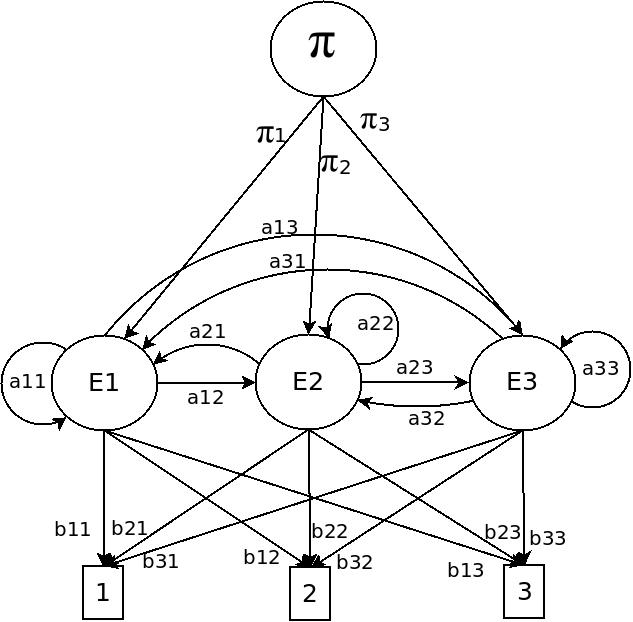
\includegraphics[scale=0.40]{imagens/HMM_exemplo.jpg}
  \caption{Grafo de um Modelo Oculto de Markov (HMM).}
  \label{img:HMM_exemplo}
\end{figure}

Existem três tipos de topologia na hora da modelagem de HMMs:

\begin{itemize}
\item \textbf{Totalmente conectada (\textit{Ergodic model}):} Todos os estados pode ser alcançado de todos os outros estados.
\item \textbf{\textit{Left-Right} (LR):} Cada estado pode voltar para si ou ir para todos os estados seguintes.
\item \textbf{\textit{Left-Right Banded} (LRB):} Cada estado pode voltar para si ou ir apenas para um estado sucessor seguinte.
\end{itemize}

A Figura \ref{img:topologias_hmm} demonstra um exemplo de grafo dessas topologias.

\begin{figure}[!htbp]
\centering
\subfigure[\textit{Ergodic model}]{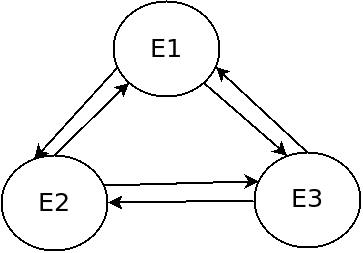
\includegraphics[width=5cm]{imagens/ergodic_HMM.jpg}}
\subfigure[\textit{Left-Right}]{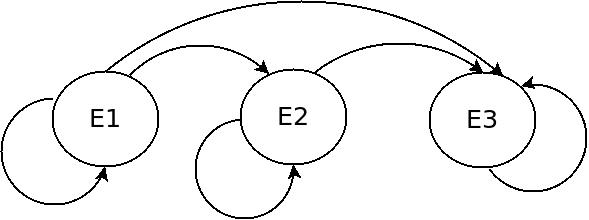
\includegraphics[width=7cm]{imagens/LR_HMM.jpg}}
\subfigure[\textit{Left-Right Banded}]{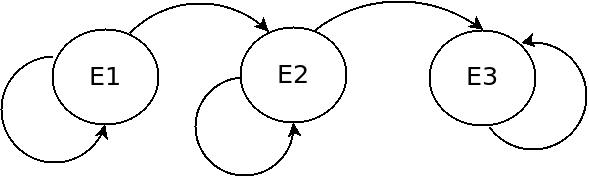
\includegraphics[width=7cm]{imagens/LRB_HMM.jpg}}
\caption{Modelos de topologias HMM.}
\label{img:topologias_hmm}
\end{figure}

Durante o processo de reconhecimento sequências de observáveis serão armazenadas para serem avaliadas em diferentes HMMs, essas sequências representam os gestos que o usuário executa diante da câmera. Para que esses gestos possam ser identificados é preciso que o sistema solucione 3 problemas: Qual a probabilidade de um gesto pertencer a uma determinada HMM, se uma gesto pertence a uma HMM qual a sequência de estados na HMM que tem a maior chance de produzi-lo e por último como estimar os parâmetros de uma HMM de forma que ela apresente a melhor probabilidade de produzir determinados tipos de gestos. Esses 3 problemas são definidos na literatura como: 

\begin{itemize}
\item \textbf{Problema 1:} Probabilidade de uma Sequência de Observáveis; como calcular de forma eficiente a probabilidade de uma sequência ser gerada por um modelo?
\item \textbf{Problema 2:} Sequência Ótima de Estados; dentre todas as diferentes sequências de estados que poderiam ter gerado uma sequência, qual é a mais provável?
\item \textbf{Problema 3:} Maximização da Probabilidade de uma Sequência de Observáveis; quais os melhores parâmetros \( \lambda = (A, B, \pi) \) do modelo para maximizar a probabilidade de uma sequência \(S\), \(P(S|\lambda)\)?
\end{itemize}

Os dois primeiros problemas podem ser resolvidos pelo algoritmo de Viterbi, o terceiro problema pode ser solucionado utilizando-se do algoritmo de Baum-Welch.


\subsection{Algoritmo de Viterbi}

Esse algoritmo é usado na resolução do problema de encontrar a sequência ótima de estados associada à seguência de observáveis. Segundo Rabiner \cite{Rabiner} é difícil decidir um critério de otimização, dentre vários que possam existir. Dessa forma a resolução desse problema poderia se dar de diferentes formas e diferentes sequências supostamente ótimas, de acordo com o critério de otimização escolhido.

 O algoritmo de Viterbi é uma solução ótima recursiva para estimar a sequência de estados em um processo de Markov de estado finito e tempo discreto. Encontrar a sequência de estados mais provável,\( E = E_1,E_2,...,E_T \), dada uma sequência de símbolos \( S = S_1,S_2,...,S_T \), ou seja, maximizar \( P(E|S,\lambda) \) equivale a maximizar \( P(E,S|\lambda) \). Ambas operações vão devolver a sequência mais provável de estados.

 Esse algoritmo funciona multiplicando os pesos das arestas anterior e próxima ao estado atual, obtendo assim sequências parciais mais prováveis. Uma escolha arbitrária acontece quando duas sequências apresentam a mesma probabilidade. Maiores informações podem ser encontradas no trabalho de Rabiner \cite{Rabiner} ou Espindola \cite{HMMLuciana}., onde o algoritmo de Viterbi para HMM é formulado. Diferentes trabalhos relacionados com o tema tiveram influência.

\subsection{Algoritmo de Baum-Welch}

Segundo \cite{Rabiner} esse é o problema mais difícil, entre os três problemas fundamentais, de resolver, porque não existe método analítico que permita que os parâmetros \( \lambda = (A, B, \pi) \) que maximizam a probabilidade de um modelo gerar uma sequência completa de símbolos observáveis, \( P(S|\lambda) \).

Contudo, o algoritmo de Baum-Welch resolve esse problema maximizando a probabilidade local. Diversos somatórios são realizados sobre o tempo de observação, $T$, com o intuito de se obter estimativas do número de vezes que cada estado é visitado em todo esse período.

Maiores detalhes como as formalizações matemáticas e o algoritmo podem ser encontrados nas obras de Rabiner \cite{Rabiner} ou Espindola \cite{HMMLuciana}.


  \Chapter{Modelo de reconhecimento de gestos}

Neste trabalho, formula-se um modelo de reconhecimento de gestos do corpo para
controle de um avatar animado em um ambiente virtual. Nesse ambiente um personagem que representa o usuário, aguarda que um gesto seja reconhecido para que ele possa executar a animação correspondente.

Para este propósito, cinco gestos foram estabelecidos: andar para direita, andar para esquerda, levantar o braço direito, levantar o braço esquerdo e levantar ambos os braços.

O modelo proposto está estruturado em cinco módulos: a captura e segmentação das imagens, a extração de características e quantização vetorial, a criação e treinamento das HMMs, a identificação das sequências de símbolos e o ambiente virtual. A Figura \ref{img:diagrama_do_sistema} exibe um diagrama do modelo proposto.

\begin{figure}[!htbp]
  \center
  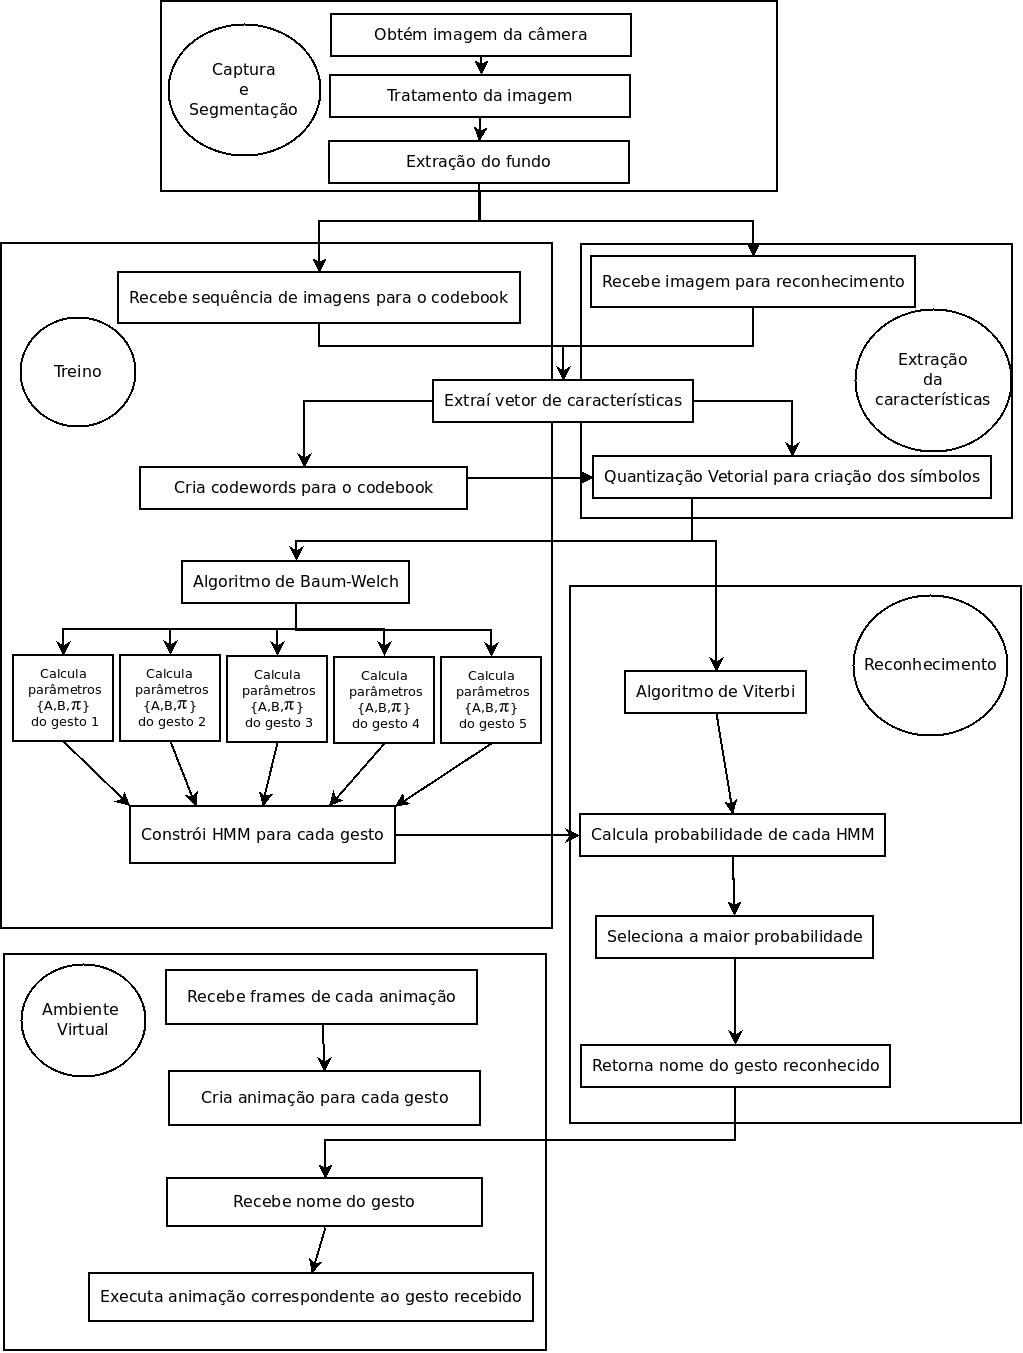
\includegraphics[scale=0.40]{imagens/diagrama_do_sistema.jpg}
  \caption{Diagrama geral do sistema.}
  \label{img:diagrama_do_sistema}
\end{figure}

No processo de captura e segmentação, foi utilizada a biblioteca OpenCV\footnote{OpenCV (Open Source Computer Vision) - http://opencv.willowgarage.com/wiki} , para obtenção de imagens a partir de uma webcam e para processamento dessas imagens com o objetivo de obter imagens binárias, neste caso com o fundo em cor preta e o usuário detectado em cor branca. Os frames \(F_i\) capturados possuem altura \(A_f\) de tamanho 640 pixels e largura \(L_f\) de 480 pixels e foram capturadas a uma taxa de 30 fps(frames por segundo).

Para que as sequências de frames possam ser aplicadas a HMMs, elas precisam ser transformadas em sequências de símbolos \(S\), portanto as imagens segmentadas são enviadas para o módulo que extrairá delas padrões de interesse segundo um algoritmo de reconhecimento de padrões, nesse caso usamos quantização vetorial, como é normalmente usado em HMMs. O espaço de características é dividido em clusters, codewords que representam os centros desses clusters são necessárias, o índice da codeword \(C_f\) é atribuído ao símbolo \(S_f\).

As características obtidas formam o vetor de características daquele frame \(V_f\). Esse vetor de características é enviado para o módulo de quantização vetorial, que retorna o índice que será usado como símbolo do grupo ao qual esse vetor foi agrupado. Para esse processo, foi utilizada a biblioteca SciPy\footnote{SciPy (Scientific Tools for Python) - http://www.scipy.org}.

No processo de modelagem, treinamento e identificação dos gestos foram utilizadas HMMs. A biblioteca GHMM\footnote{GHMM (General Hidden Markov Model library) - http://ghmm.org} foi utilizada para esse propósito.

De cada gesto foram gravados cinco vídeos, executando os gestos de forma um pouco diferente, quatro desses vídeos foram usados para o treinamento de suas respectivas HMMs, esse treino foi feito utilizando-se os valores dos índices retornados pela quantização vetorial do vetor de características de cada frame desses vídeos. O quinto vídeo foi gravado com o propósito de testar os modelos.

Durante a execução em tempo real de identificação dos gestos, a cada segundo de vídeo, uma sequência de índices é avaliada em cada um dos cinco modelos ocultos de Markov e a probabilidade dessa sequência pertencer ao modelo é armazenada. O gesto reconhecido será aquele representado pelo modelo que retornou a probabilidade mais alta.

O gesto identificado ativa uma função que executa a animação correspondente do avatar no ambiente virtual, dentro de um conjunto de animações possíveis previamente criadas.

\section{Captura e segmentação}

No processo de captura, as imagens são capturas em uma taxa de 30 frames por segundo, através da biblioteca OpenCV. OpenCV é uma biblioteca de visão computacional, escrita em C e C++ e roda em Linux, Windows e Mac OS X. Com interface para linguagens como Python, Ruby, Matlab e outras. OpenCV foi projetada para eficiência e aplicativos em tempo real, usar vantagens de processadores com vários núcleos. A biblioteca contém mais de 500 funções que se espalham por várias áreas de visão computacional,
além de módulos de processamento de imagem e vídeo I/O, estrutura de dados, álgebra linear,
GUI (Inteface Gráfica do Usuário) básica com sistema de janelas independentes, controle de
mouse e teclado, calibração de câmera, reconhecimento de objetos e análise estrutural e
é um software aberto ao uso acadêmico e comercial \cite{LearningOpenCV}.

As imagens são pré-processadas com as funções de OpenCV para poder, finalmente, ter características extraídas.

\subsection{Extração do fundo}

No início do módulo de captura, é necessário que o sistema armazene uma imagem do fundo do ambiente, ela será utilizada durante o processo de extração do fundo.

Todos os frames seguintes sofrem uma operação de subtração em relação ao frame de fundo.
A imagem resultante passará por um processo de binarização segundo uma tolerância, que dita a partir de quanta diferença os pixels devem ser considerados brancos, todos os pixels que ficarem abaixo dessa diferença serão pretos. A Figura \ref{img:processo_segmentacao} demonstra um exemplo de processo de  subtração de fundo do sistema.

\begin{figure}[!htbp]
\center
\subfigure[img:fundo][Fundo]{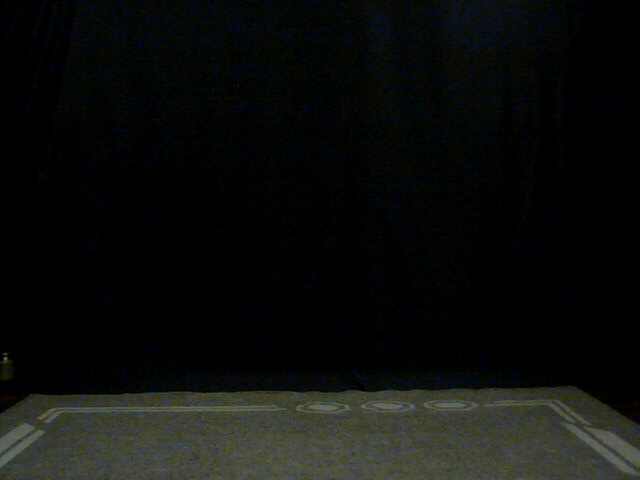
\includegraphics[width=5cm]{imagens/fundo.jpg}}
\qquad
\subfigure[img:frame][Imagem]{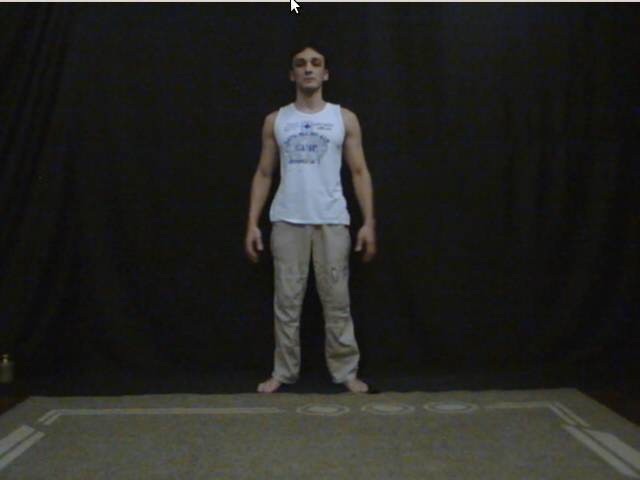
\includegraphics[width=5cm]{imagens/frame.jpg}}
\qquad
\subfigure[img:mascara][Subtração]{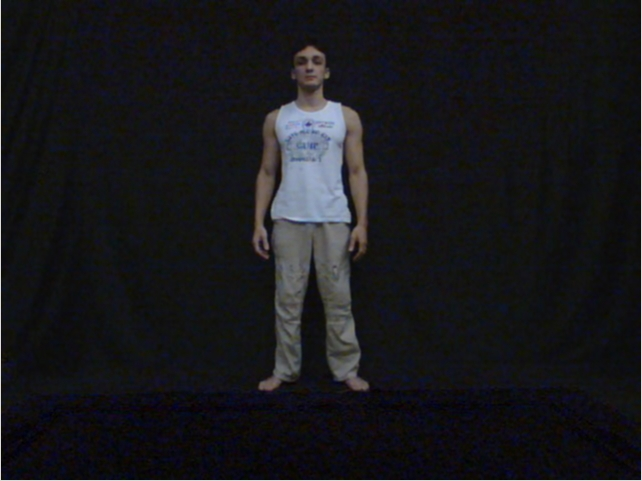
\includegraphics[width=5cm]{imagens/mascara.jpg}}
\qquad
\subfigure[img:binario][Binário]{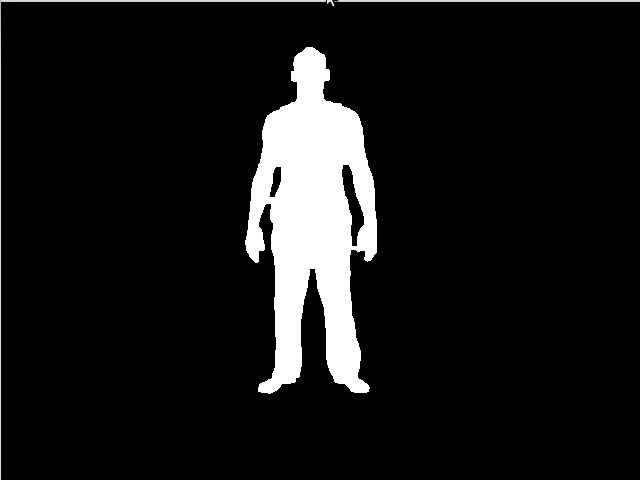
\includegraphics[width=5cm]{imagens/binario.jpg}}
\caption{Processo de segmentação}
\label{img:processo_segmentacao}
\end{figure}



\subsection{Processamento das imagens}

É importante realizar alguns pré-processamentos e pós-processamentos nas imagens com o intuito de melhorar a silhueta detectada e remover ruídos e informações desnecessárias. Esses processamentos são operações morfológicas, suavização e eliminação de falsas detecções.

\subsubsection{A) Remoção de ruídos}

Todos os frames capturados, inclusive a imagem de fundo, são tratados com filtro de gauss com objetivo de suavizar as imagens, removendo assim, ruídos da imagem antes de sofrerem o processo de subtração, a Figura \ref{img:gauss_process} demonstra o efeito do filtro de Gauss com kernel de tamanho $3\times3$ no processo de eliminação de pequenos ruídos, esses efeitos não ficaram tão evidentes porque nos ambientes onde as gravações foram feitas havia condições ideais de iluminação, a câmera estava adequadamente configurada e o fundo era completamente estático e simples.

\begin{figure}[!htbp]
\subfigure[img:arms_up][Imagem]{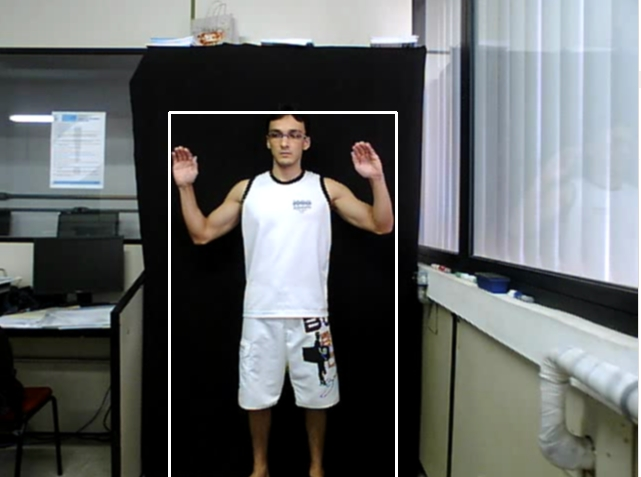
\includegraphics[width=5cm]{imagens/arms_up.jpg}}
\subfigure[img:no_gauss][Antes do filtro]{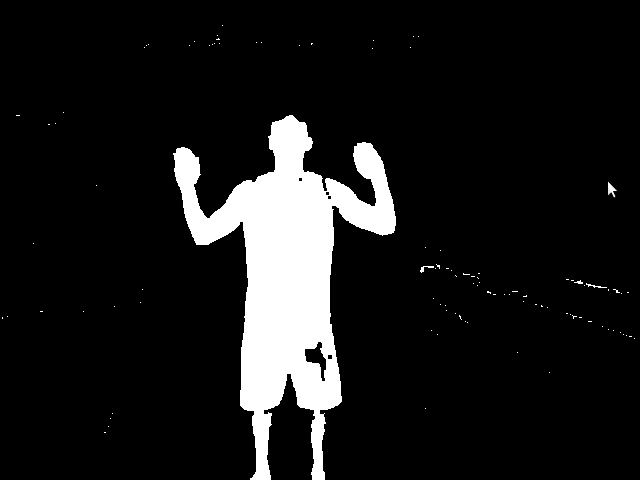
\includegraphics[width=5cm]{imagens/no_gauss.jpg}}
\subfigure[img:gauss][Após o filtro]{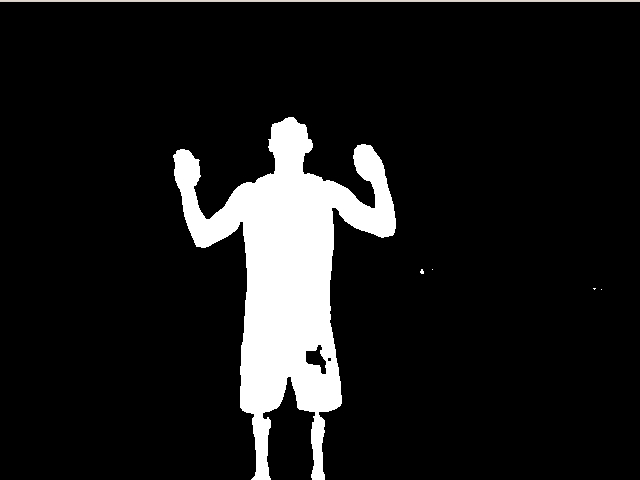
\includegraphics[width=5cm]{imagens/gauss.jpg}}
\caption{Pequenos ruídos sendo eliminados pelo filtro de Gauss}
\label{img:gauss_process}
\end{figure}

\subsubsection{B) Operações morfológicas}

Um filtro de dilatação (\textit{dilate}), que expande os pixels na imagem, foi aplicado na imagem binária, com a intenção de remover falhas no interior da silhueta, em conjunto com um filtro de erosão (\textit{erode}), em seguida, para transformar a silhueta dilatada, mas sem essas falhas, na silhueta com tamanho normal. Através da Figura \ref{img:dilate_erode} é possível observar pequenos espaços dentro da silhueta sendo conectados pelo processo de dilatação e gerando uma silhueta maior do que a primeira e esse efeito sendo atenuado pelo filtro de erosão. O resultado é uma silhueta próxima a original, mas sem as falhas internas.

\begin{figure}[!htbp]
\subfigure[img:arms_up][Imagem]{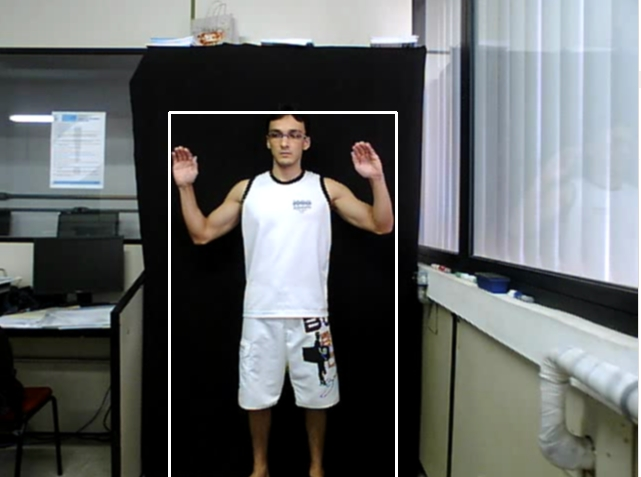
\includegraphics[width=5cm]{imagens/arms_up.jpg}}
\subfigure[img:dilate][\textit{Dilate}]{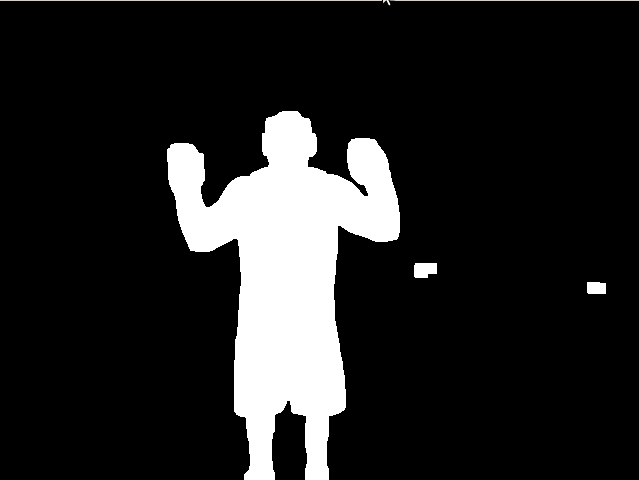
\includegraphics[width=5cm]{imagens/dilate.jpg}}
\subfigure[img:erode][\textit{Erode}]{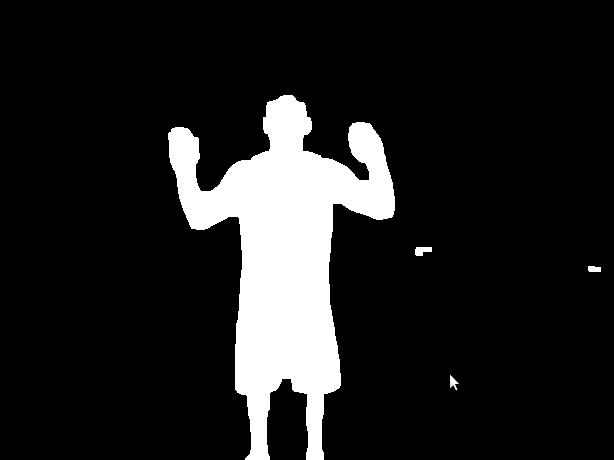
\includegraphics[width=5cm]{imagens/erode.jpg}}
\caption{Filtros de dilatação e erosão criam uma silhueta sem falhas no interior.}
\label{img:dilate_erode}
\end{figure}


\subsection{Eliminação de detecções desnecessárias}

Com a imagem binária, funções que criam contornos retangulares aos redores das formas detectadas foram usadas com o intuito de marcar os objetos de interesse. Na Figura \ref{img:maior_forma} é perceptível que mais de uma forma, como por exemplo sombras ou outras pessoas, pode ser detectada em um mesmo frame e é preciso que apenas uma forma seja levada em consideração por frame, por isso a área de cada um dos retângulos foi calculada e apenas o maior deles foi copiado para uma imagem contendo as dimensões desse retângulo, chamada de região de interesse.

\begin{figure}[!htbp]
\center
\begin{tabular}{ccc}
\subfigure{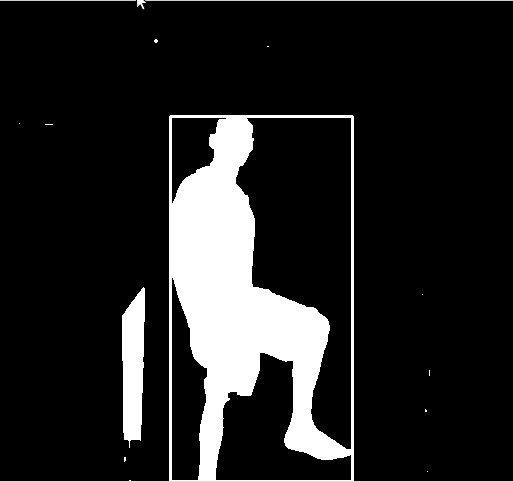
\includegraphics[scale=0.25]{imagens/maior_forma.jpg}} & \hspace{0.5cm} &
\subfigure{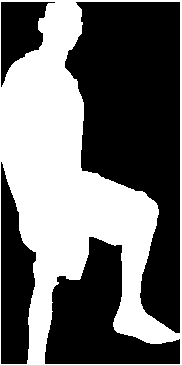
\includegraphics[scale=0.25]{imagens/maior_forma_2.jpg}} \\
Todos os contornos & & Contorno avaliado  
\end{tabular}
\caption{Quando mais de um contorno é detectados em um mesmo frame, apenas o maior é avaliado.}
\label{img:maior_forma}
\end{figure}

\section{Modelo do vetor de características}

Para formação do vetor de características \(V_f\) usou-se características de malha, por sua capacidade de descrever complexos padrões em duas dimensões com sucesso, cada imagem (\(L_f\times{A_f}\) pixels) contendo a região de interesse é dividida em segmentos de malha de tamanho \(L_s\times{A_s} \) pixels. A proporção de pixels brancos em cada malha se torna um elemento do vetor de características de acordo com,

\[V_{(i+j)} = \frac{pixelsBrancos_{(ij)}}{L_s\times{A_s}}\].

Onde $pixelsBrancos_{(ij)}$ é o número de pixels brancos no segmento $i,j$. A malha utilizada no começo do sistema tinha tamanho $3\times3$, gerando um vetor de características de tamanho 9, esse tamanho não gerou informações suficientes para diferenciar bem algumas posturas como, por exemplo, estar virado para direita ou para esquerda, gerando bastante confusão quando se estava nessas posições, aumentar a malha resolveu esse problema.
Apesar de \cite{YAMATO} terem divido os segmentos da malha em partes de $8\times8$ pixels, gerando um vetor de características de dimensão 625, esse valores pareceram excessos desnecessários, ter dobrado a altura e largura da malha no sistema  foi suficiente para os problemas de confusão nas posturas. A Figura \ref{img:malha} exibe um exemplo de malha de características de tamanho $6\times6$, utilizada no sistema final, ela gera um vetor de tamanho 36. A Tabela \ref{table:valores_malha} demonstra exemplo de valores dessas características no caso de uma malha $ 3\times{3}$ .

A biblioteca SciPy foi usada durante esse procedimento. SciPy é uma biblioteca de Open Source de ferramentas científicas para Python, ela depende da Biblioteca NumPy, que é uma biblioteca para linguagem Python que permite trabalhar com vetores e matrizes de uma forma comparável e com uma sintaxe semelhante ao software proprietário Matlab, mas com muito mais eficiência e com toda a expressividade da linguagem. SciPy reúne uma variedade de módulos para estatística, transformadas de Fourier, álgebra linear, processamento de sinais e imagens, etc.

\begin{figure}[!htbp]
  \center
  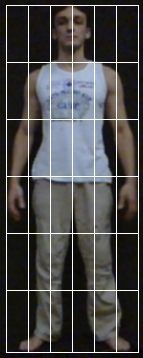
\includegraphics[scale=0.40]{imagens/malha.jpg}
  \caption{Uma malha de características de tamanho $6\times6$.}
  \label{img:malha}
\end{figure}

\begin{table}[!htbp]
\caption{Exemplos de valores de uma malha de características, 1.0 significa que o segmento da malha é todo branco e 0.0 significa que o segmento é todo preto.}
\label{table:valores_malha}
\centering
\begin{tabular}{p{4.5cm} | p{4.5cm} | p{4.5cm}}
\toprule
\small{0.27971014492753621} & \small{0.85797101449275359} & \small{0.36935817805383026} \\ \midrule
\small{0.65051759834368528} & \small{0.99109730848861288} & \small{0.74824016563147} \\ \midrule
\small{0.33830227743271224} & \small{0.44761904761904764} & \small{0.59565217391304348}\\
\bottomrule
\end{tabular}
\end{table}

\subsection{Modelo de reconhecimento de padrões}

Para o processo de reconhecimento de padrões, o método de clusterização por k-means \cite{Patter-Recognition-M-Bishop} foi utilizado. O algoritmo recebe como entrada o número de clusters \(K\) e a matriz de todos os vetores de características do treino e como saída gera os vetores de características que representam os centros desses clusters. Um vetor \(V\) pertence ao cluster \(C\) se ele está mais perto do centro de \(C\) do que quaisquer outros centros dos outros clusters. Se \(V\) for agrupado ao cluster \(C\), dizemos que o cluster \(C\) é o centro dominante de \(V\).

O algoritmo k-means realiza varias iterações para convergir para um mínimo local, em função das distâncias entre cada vetor e os centros de todos os clusters. Em geral, a convergência pode ser relativamente lenta se número de vetores e número $K$ for grande, mas neste caso o número $K$ é pequeno e o número de vetores é relativamente pequeno, por tanto será rápida a convergência. Uma boa escolha dos centros iniciais é fundamental neste método para se obter resultados eficientes. Neste caso, é escolhido como centros iniciais um conjunto de imagens representativas de cada gesto, por tanto seus respectivos vetores de características são considerados como centros iniciais. Isso garante um resultado confiável do processo de clusterização. Uma vez definidos os $K$ centros, se atribue cada vetor de características ao cluster para o qual a distância entre esse vetor e o centro desse cluster é menor que a de todos os outros clusters. Uma vez concluída a distribuição dos vetores característicos em diferentes clusters, é calculado o novo centro de cada cluster como a média aritmética de seus elementos. Se existir alguma variação entre os centros novos e os anteriores, os novos centros passam a ser os $K$ centros para uma nova iteração de clusterização, ignorando os anteriores. Esse processo é realizado enquanto houver alguma variação entre os respectivos centros, caso contrário acontece a convergência. O conjunto de $K$ centros da convergência são os vetores dominantes, que representam a os vetores característicos de seus respectivos clusters \cite{Liu}.

Todos os próximos vetores de características serão classificados de acordo com o número do cluster (também chamado de índice centróide ou índice do centro mais próximo) ao qual ele foi agrupado. Assim, por exemplo, na fase de treino, os $N_j$ vetores que pertencem ao cluster $C_j$ se identificam com o índice $j$. Na fase de reconhecimento, qualquer vetor característico da imagem em análise será testado com todos os clusters por proximidade. O índice do cluster mais próximo será atribuído como índice do vetor para ser classificado pelo modelo HMM correspondente.

O algoritmo de quantização, neste caso usando o algoritmo k-means, tenta minimizar a distorção, que é definido como a soma do quadrado das distâncias entre cada vetor de características e seu centro dominante e retorna um conjunto de índice de centros, um para cada vetor de características, esses índices serão utilizados como símbolos para as HMMs. Exemplo, para $K$ clusters, o índice das imagens que correspondem aos clusters $C_j$ é $j$, para $j = 1, ..., K$.

Neste trabalho, cada um dos 5 gestos é representado por uma sequência de $p$ frames, portanto são em total $5p$ imagens (seus respectivos vetores característicos) que devem ser clusterizados. Considera-se 4 posturas representativas que definem eficientemente cada gesto, em consequência serão $4 \times 5 = 20$ centros e 1 postura considerada default (postura parado de frente para a câmera), que implicam a definição de 21 clusters. No processo de clusterização por k-means, os 21 centros iniciais foram especificados por concepção visual de representação da postura. No final de cada processo os centros determinados nem sempre são as definidas inicialmente e possivelmente não exista uma imagem associada ao centro, devido ao fato de que em cada iteração do k-means os novos centros são determinados como a média aritmética dos elementos dos clusters.

Na Figura \ref{img:centros_clusters} se exibem as imagens centros iniciais das posturas de cada gesto. A Tabela \ref{table:codebook} exibe a estrutura do codebook, onde a posição 0 é usada para o cluster que representa a imagem parado virado de frente para câmera, os índices de 1 a 4 são escolhidos para a seqûencia de posturas que definem o gesto de dar um passo para a direita, os índices de 5 a 8 as posturas escolhidas para definir o gesto de dar um passo para a esquerda, 9 a 12 o gesto de levantar o braço direito, 14 a 16 levantar o braço esquerdo e 17 a 20 para representar o gesto de levantar ambos os braços. Dessa forma um total de 21 índices foram definidos.

A Figura \ref{img:agrupamentos} exibe alguns resultados de agrupamentos, onde todas as imagens à esquerda da seta nas figuras retornam um mesmo símbolo, o índice do centro do cluster ao qual elas foram agrupadas, representado pelo número exibido a direita das setas nas figuras, as imagens a direita da seta foram utilizadas para terem seu vetores de características extraídos para representar o centro inicial dos respectivos clusters.

\begin{table}[!htbp]
\caption{Estrutura do Codebook.}
\label{table:codebook}
\centering
\begin{tabular}{p{4.5cm} | p{6.5cm}}
\toprule
\textbf{Índice/Símbolo} & \textbf{Codeword} \\
\midrule[1pt]
0 & Parado virado de frente para câmera \\ \midrule
1 & Passo para direita 1 \\ \midrule
2 & Passo para direita 2 \\ \midrule
3 & Passo para direita 3 \\ \midrule
4 & Passo para direita 4 \\ \midrule
5 & Passo para esquerda 1 \\ \midrule
6 & Passo para esquerda 2 \\ \midrule
7 & Passo para esquerda 3 \\ \midrule
8 & Passo para esquerda 4 \\ \midrule
9 & Levantar braço direito 1 \\ \midrule
10 & Levantar braço direito 2 \\ \midrule
11 & Levantar braço direito 3 \\ \midrule
12 & Levantar braço direito 4 \\ \midrule
13 & Levantar braço esquerdo 1 \\ \midrule
14 & Levantar braço esquerdo 2 \\ \midrule
15 & Levantar braço esquerdo 3 \\ \midrule
16 & Levantar braço esquerdo 4 \\ \midrule
17 & Levantar ambos os braços 1 \\ \midrule
18 & Levantar ambos os braços 2 \\ \midrule
19 & Levantar ambos os braços 3 \\ \midrule
20 & Levantar ambos os braços 4 \\
\bottomrule
\end{tabular}
\end{table}

\begin{figure}[!htbp]
\center
\begin{tabular}{ccccccc}
	
\subfigure{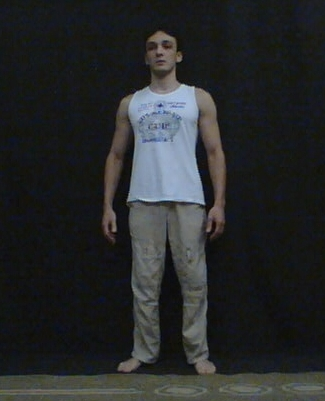
\includegraphics[scale=0.23]{imagens/codeword_parado.jpg}}
\\
(0)
\\
\subfigure{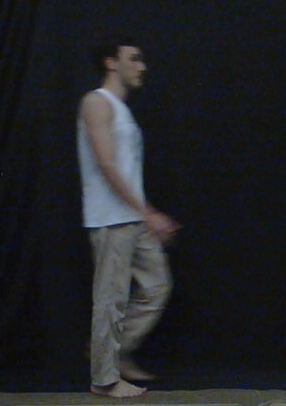
\includegraphics[scale=0.23]{imagens/codewords_passo_direita_1.jpg}} & \hspace{0.5cm} &
\subfigure{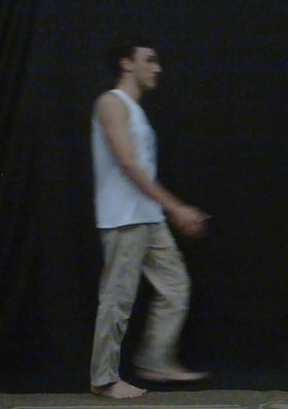
\includegraphics[scale=0.23]{imagens/codewords_passo_direita_2.jpg}} & \hspace{0.5cm} &
\subfigure{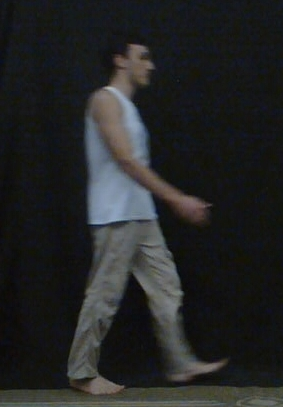
\includegraphics[scale=0.23]{imagens/codewords_passo_direita_3.jpg}} & \hspace{0.5cm} &
\subfigure{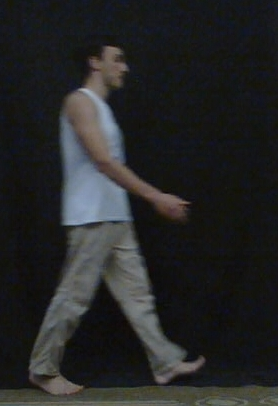
\includegraphics[scale=0.23]{imagens/codewords_passo_direita_4.jpg}}
\\
(1) & & (2) & & (3) & & (4) 
\\
\subfigure{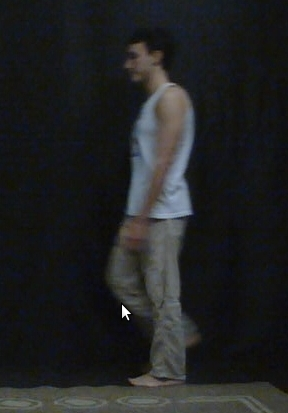
\includegraphics[scale=0.23]{imagens/codewords_passo_esquerda_1.jpg}} & &
\subfigure{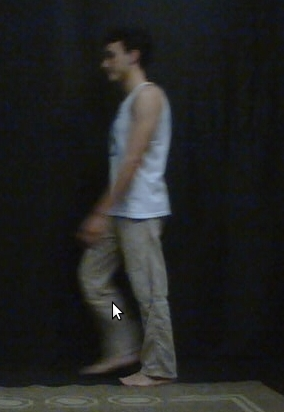
\includegraphics[scale=0.23]{imagens/codewords_passo_esquerda_2.jpg}} & &
\subfigure{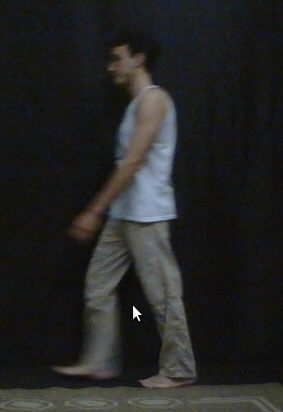
\includegraphics[scale=0.23]{imagens/codewords_passo_esquerda_3.jpg}} & &
\subfigure{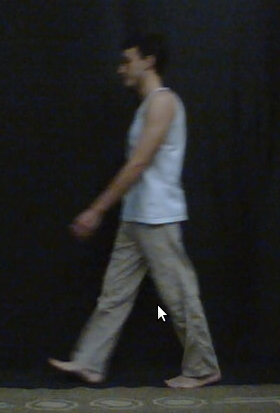
\includegraphics[scale=0.23]{imagens/codewords_passo_esquerda_4.jpg}}
\\
(5) & & (6) & & (7) & & (8) 
\\
\subfigure{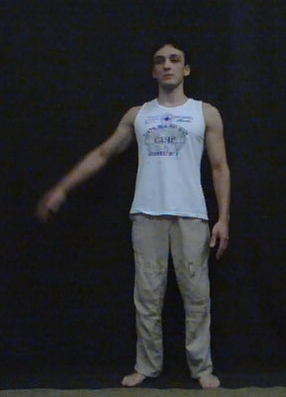
\includegraphics[scale=0.23]{imagens/codewords_braco_direito_1.jpg}} & &
\subfigure{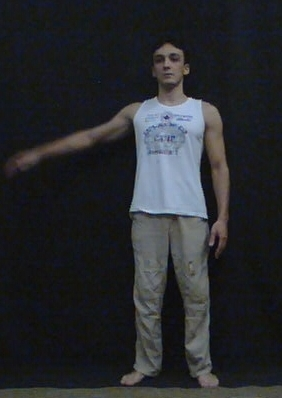
\includegraphics[scale=0.23]{imagens/codewords_braco_direito_2.jpg}} & &
\subfigure{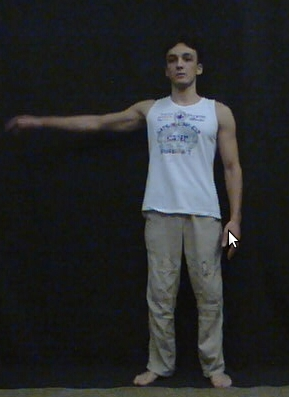
\includegraphics[scale=0.23]{imagens/codewords_braco_direito_3.jpg}} & &
\subfigure{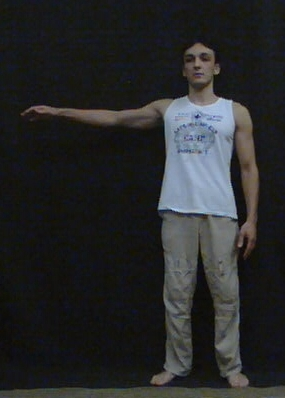
\includegraphics[scale=0.23]{imagens/codewords_braco_direito_4.jpg}}
\\
(9) & & (10) & & (11) & & (12) 
\\
\subfigure{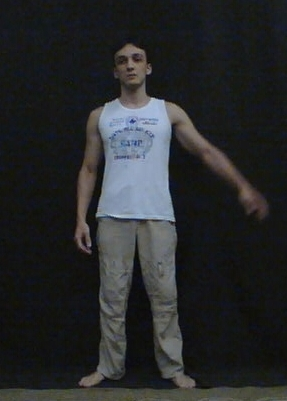
\includegraphics[scale=0.23]{imagens/codewords_braco_esquerdo_1.jpg}} & &
\subfigure{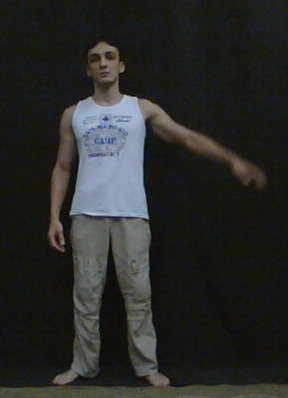
\includegraphics[scale=0.23]{imagens/codewords_braco_esquerdo_2.jpg}} & &
\subfigure{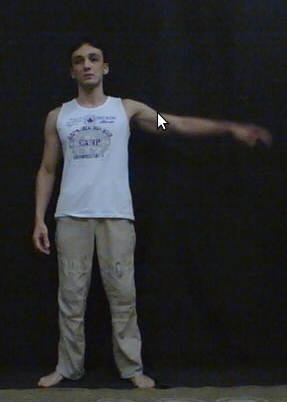
\includegraphics[scale=0.23]{imagens/codewords_braco_esquerdo_3.jpg}} & &
\subfigure{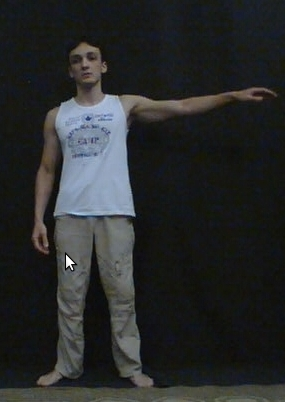
\includegraphics[scale=0.23]{imagens/codewords_braco_esquerdo_4.jpg}}
\\
(13) & & (14) & & (15) & & (16) 
\\
\subfigure{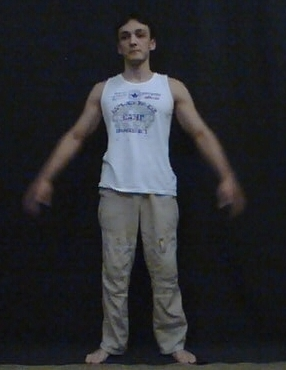
\includegraphics[scale=0.23]{imagens/codewords_2_bracos_1.jpg}} & &
\subfigure{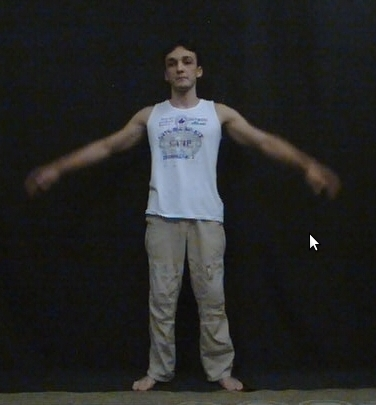
\includegraphics[scale=0.23]{imagens/codewords_2_bracos_2.jpg}} & &
\subfigure{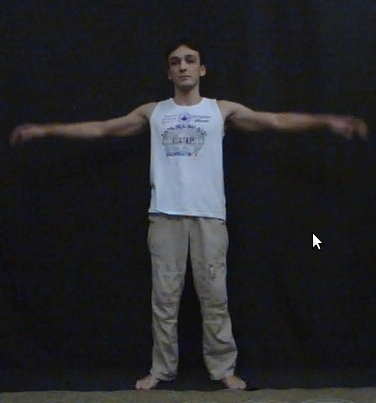
\includegraphics[scale=0.23]{imagens/codewords_2_bracos_3.jpg}} & &
\subfigure{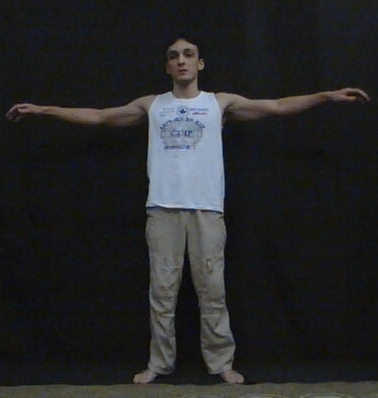
\includegraphics[scale=0.23]{imagens/codewords_2_bracos_4.jpg}}
\\
(17) & & (18) & & (19) & & (20) 

\end{tabular}
\caption{Imagens representativas dos centros dos clusters.}
\label{img:centros_clusters}
\end{figure}

\begin{figure}[!htbp]
  \center
  \subfigure{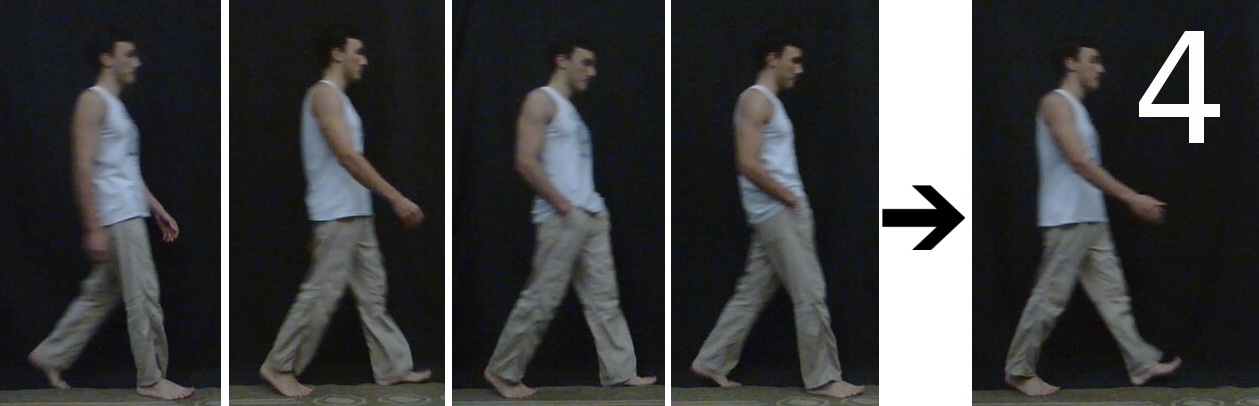
\includegraphics[width=12cm]{imagens/exemplo_vq_4.jpg}}
  \qquad
  \subfigure{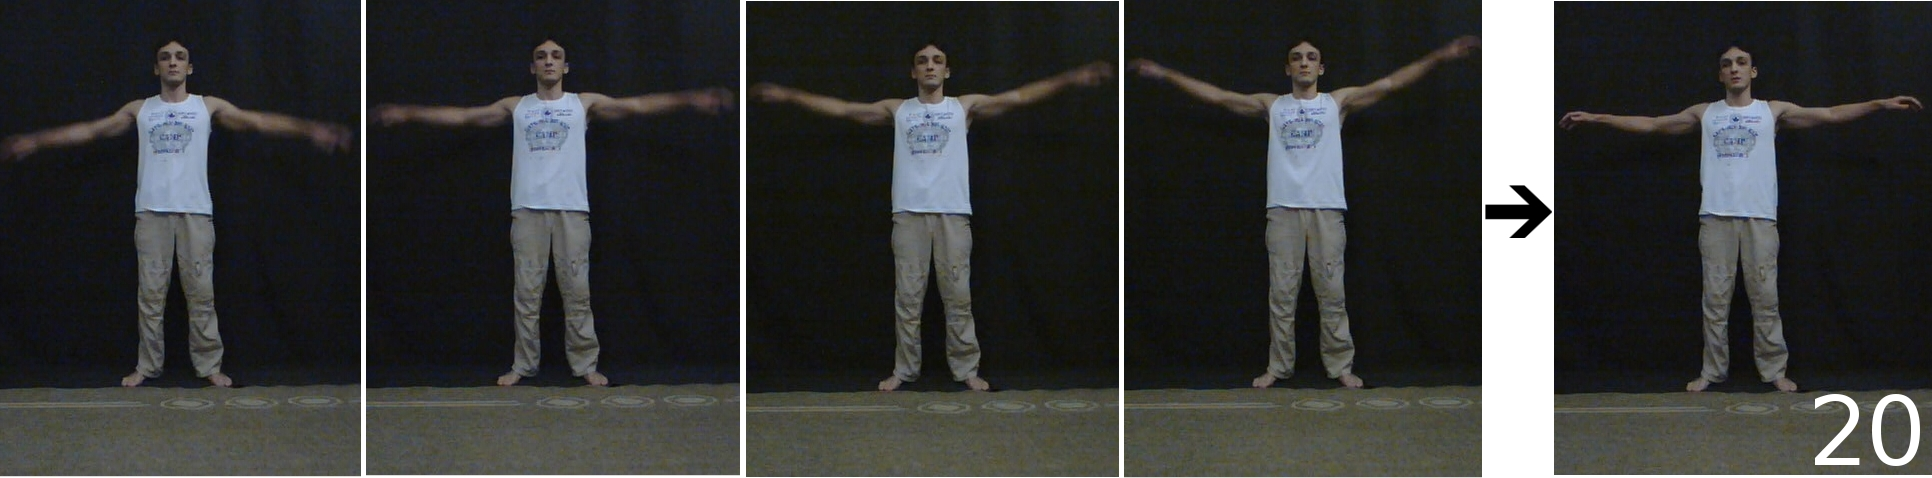
\includegraphics[width=12cm]{imagens/exemplo_vq_20.jpg}}
  \caption{As imagens a esquerda da seta foram agrupadas ao cluster de índice representado pelo número a direita da seta, todas elas serão representadas pelo símbolo correspondente a esse número nas HMMs.}
  \label{img:agrupamentos}
\end{figure}


\section{Modelagem das HMMs}

Liu et al. \cite{UnderstandingHMMTrainingForVideoGestureRecognition}, Elmezain et al. \cite{HMM-Based_Isolated_Hand_Gesture_Recognition} e Tataru et al. \cite{OnHandGesturesRecognitionUsingHiddenMarkovModels} chegaram a conclusão de que a topologia LRB (\textit{Left Right Banded}) como modelo na HMM apresenta a melhor taxa de reconhecimento. Por isso essa foi a topologia utilizada no início do sistema. A biblioteca GHMM auxiliou no processo de modelagem, treino e reconhecimento das sequências de entrada.

A topologia LRB, para o propósito deste trabalho é de quatro estados com arestas de transição entre estados adjacentes de esquerda para direita, com ciclos nos mesmos estados, tal como ilustra a Figura \ref{img:HMM_sistema}, cuja matriz de transições $A$ deve ser da seguinte forma:

\begin{equation}\label{matriz_A}
  A =
    \begin{pmatrix}
      a_{11} & 1-a_{11} & 0 & 0 \\
      0 & a_{22} & 1-a_{22} & 0 \\
      0 & 0 & a_{33} & 1-a_{33}  \\
      0 & 0 & 0 & 1
    \end{pmatrix}
\end{equation}

\begin{figure}[!htbp]
  \center
  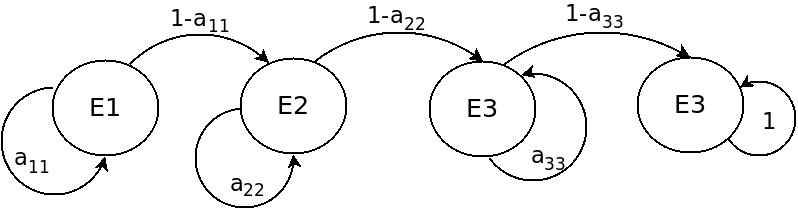
\includegraphics[scale=0.40]{imagens/HMM_sistema.jpg}
  \caption{Aplicação da matrix $A$ na topologia LRB.}
  \label{img:HMM_sistema}
\end{figure}

Durante o processo de criação da HMM $\lambda$ é necessária a inicialização do valores $\lambda(A, B, \pi)$. Segundo \cite{UnderstandingHMMTrainingForVideoGestureRecognition}, a matriz \(A\) nessa topologia é inicializada através da computação da duração \(d\) do estado de acordo com
\[d = \frac{T}{N}\], onde \(N\) é número de estados da HMM e \(T\) é o tamanho da duração do gesto. A taxa de imagens gravadas pela câmera é de 30 frames por segundo, o sistema foi projetado para a cada segundo enviar os últimos 30 símbolos para serem avaliados em cada HMM, portanto o valor de $T = 30$ nesse sistema. O número de estados que cada HMM contém é 4, devido ao fato de que cada gesto possui 4 símbolos. Essa duração segmenta a sequência de observação uniformemente; portanto cada estado possui a mesma duração, nesse caso \(d\) equivale a \( 30/4 = 7.5\), dai que \(a_{ii} = 1/d\), logo a matriz \(A\) associada à Figura \ref{img:HMM_sistema}, segundo (\ref{matriz_A}), é inicializada da seguinte forma

\[
 A =
 \begin{pmatrix}
  0.75 & 0.25 & 0 & 0 \\
  0 & 0.75 & 0.25 & 0 \\
  0 & 0 & 0.75 & 0.25  \\
  0 & 0 & 0 & 1
 \end{pmatrix}.
\]

O segundo parâmetro a ser inicializado é a matriz \(B\), os estados de uma cadeia HMM são discretos, portanto todos os elementos da matriz \(B\) podem ser inicializados com o mesmo valor para todos os estados. A matriz \(B\) será inicializada da seguinte forma 
\[B = \{b_{im}\}, \mbox{ para } b_{im} = \frac{1}{M}, \mbox{ onde } 1 \leq i \leq N, 1 \leq m \leq M; \] 
sendo \(N\) o número de estados e \(M\) a quantidade de símbolos, tal como foi estabelecido anteriormente na sessão \ref{hmm}. O terceiro parâmetro é o vetor \(\pi\), que assumirá

\[
 \pi =
 \begin{pmatrix}
  1 & 0 & 0 & 0
 \end{pmatrix},
\]
porque deve-se garantir que a HMM sempre começá pelo primeiro estado. A Figura \ref{img:HMM_antes_treino} demonstra o grafo das HMMs criadas utilizando-se os parâmetros acima.

\begin{figure}[!htbp]
  \center
  \caption{HMMs antes do processo de treino.}
  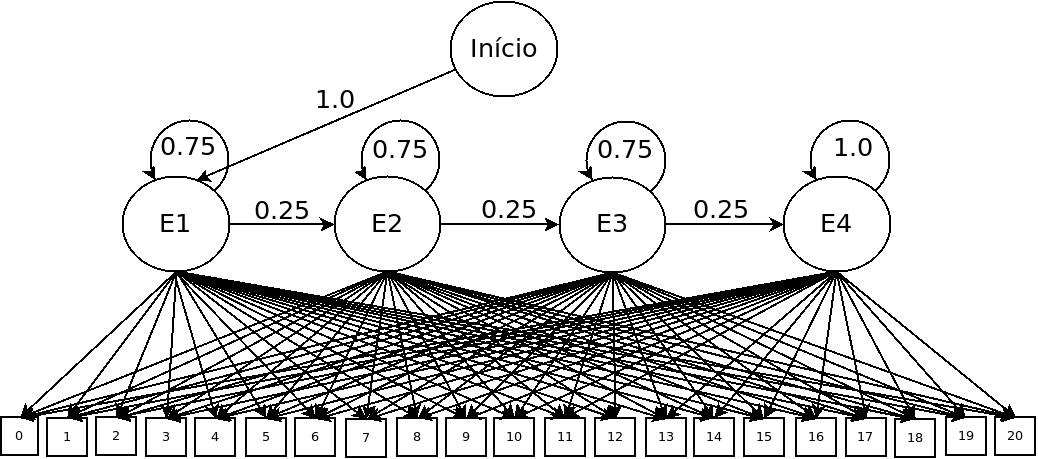
\includegraphics[scale=0.40]{imagens/HMM_antes_treino.jpg}
  \label{img:HMM_antes_treino}
\end{figure}

\subsection{Processo de treinamento}

Os símbolos de saída da quantização vetorial precisam ser armazenados em um vetor, para serem posteriormente avaliados pelo algoritmo de Viterbi. No trabalho de Elmezain et al. \cite{HMM-Based_Isolated_Hand_Gesture_Recognition}, o sistema foi projetado para reconhecer gestos com significados a partir da detecção da codeword zero. Isso significa que o vetor de símbolos começa a ser construído a partir do momento que um símbolo zero é reconhecido e o final desse vetor acontece quando outro símbolo zero é identificado.

Se fosse implementar esse modelo nesse sistema, uma postura específica para ser representada pela codeword zero haveria de ser criada e todos os meus gestos começariam e terminariam com essa postura, seria importante que essa postura também não aparecesse durante os gestos para que os mesmos não tivessem seus vetores interrompidos.

Essa postura no começo e no fim dos gestos não tornaria a interação tão natural quanto se pudéssemos implementar um sistema onde ela não fosse necessária, por esse motivo, esse sistema funciona enviando a cada segundo, todos os símbolos reconhecidos nesse tempo. Já que a câmera que foi utilizada captura trinta imagens por segundo, trinta símbolos são armazenados e enviados para o módulo de reconhecimento a cada segundo.

Seria ideal que cada um dos quatro estados da HMM retornasse apenas um dos quatro símbolo de cada gesto. Se não houvesse ruídos ou erros de distorções, em condições ideais cada segundo de vídeos produziria uma sequência parecida com, por exemplo; \[[1,1,1,1,1,1,1,1,2,2,2,2,2,2,2,3,3,3,3,3,3,3,4,4,4,4,4,4,4,4]\].
Essa sequência seria facilmente reconhecida como "passo a direita" pela classificação de uma HMM configurada para produzir a maior probabilidade desses símbolos aparecerem nessa ordem. Essa HMM ideal é representada na Figura \ref{img:HMM_1_ideal}.

\begin{figure}[!htbp]
  \center
  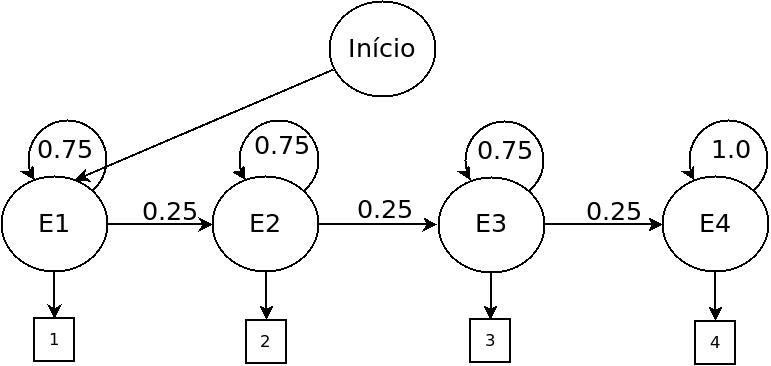
\includegraphics[scale=0.35]{imagens/HMM_1_ideal.jpg}
  \caption{Parâmetros de uma HMM configurada para reconhecer um passo a direita, se não houvesse ruído e/ou erro.}
  \label{img:HMM_1_ideal}
\end{figure}

Na realidade isso não acontece e um único símbolo errado ou com distorção maior, comprometeria todo o processo de reconhecimento. Por exemplo, de sequência para ser reconhecida pelo sistema poderia ser
\[[17, 1, 1, 1, 2, 2, 3, 3, 3, 3, 4, 4, 4, 4, 4, 4, 17, 1, 1, 1, 2, 2, 2, 3, 3, 3, 3, 4, 4, 4]\]
que se aproxima mais do gesto um "passo a direita" do que todos os outros, por conter a maior parte de símbolos associados a esse gesto, o sistema deve ser capaz de lidar com essas variações e ainda assim fazer identificações correta.

É inviável tentar estimar os melhores valores (ótimos) para as parâmetros \((A, B, \pi)\). Na verdade, o problema de treinar um grafo desta característica com valores exatos é um problema difícil, por tanto se recorre a métodos de aproximação como Baum-welch o qual o resultado é uma convergência local. Nesse sentido, para treino de HMM o algoritmo de Baum-welch é utilizado recebendo como entrada as sequências de símbolos extraídas de cada um dos quatro vídeos gravados de cada um dos gestos. Para cada um dos 5 gestos é gerado um modelo HMM a partir do modelo inicial proposto e considerando que todos os estados possuem saídas para todos os símbolos, tal como mostrado na Figura \ref{img:HMM_antes_treino}. Os modelos gerados são $\lambda_1, \lambda_2, \lambda_3, \lambda_4$ e $\lambda_5$, os quais são mostrados pelas figuras \ref{img:HMM_5_apos_treino}, \ref{img:HMM_4_apos_treino}, \ref{img:HMM_3_apos_treino}, \ref{img:HMM_2_apos_treino} e \ref{img:HMM_1_apos_treino}, respectivamente.

\begin{figure}[!htbp]
  \center
  \caption{Parâmetros de uma HMM treinada com os vídeos do gesto levantar ambos os braços.}
  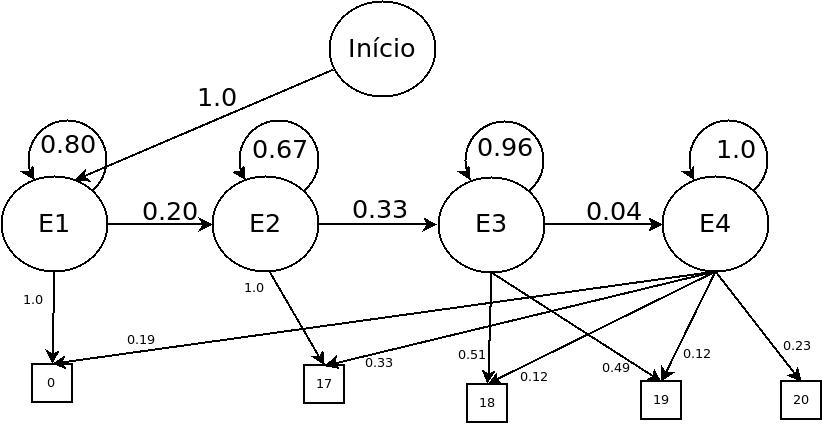
\includegraphics[scale=0.35]{imagens/HMM_5_apos_treino.jpg}
  \label{img:HMM_5_apos_treino}
\end{figure}

\begin{figure}[!htbp]
  \center
  \caption{Parâmetros de uma HMM treinada com os vídeos do gesto levantar o braço esquerdo.}
  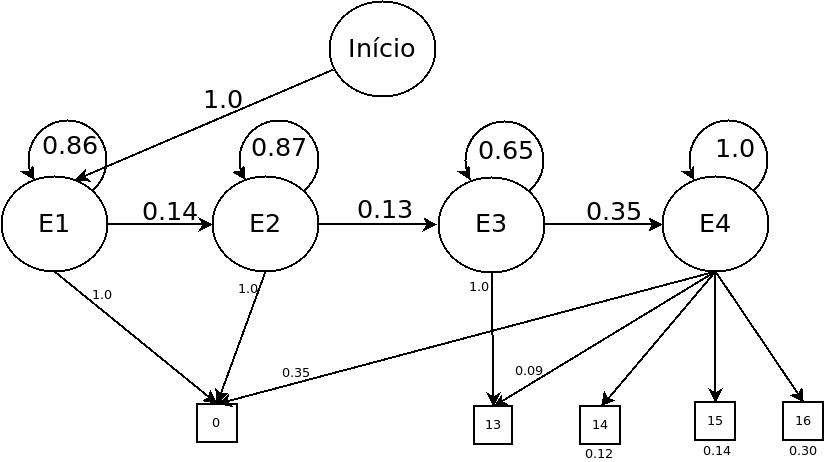
\includegraphics[scale=0.35]{imagens/HMM_4_apos_treino.jpg}
  \label{img:HMM_4_apos_treino}
\end{figure}

\begin{figure}[!htbp]
  \center
  \caption{Parâmetros de uma HMM treinada com os vídeos do gesto levantar o braço direito.}
  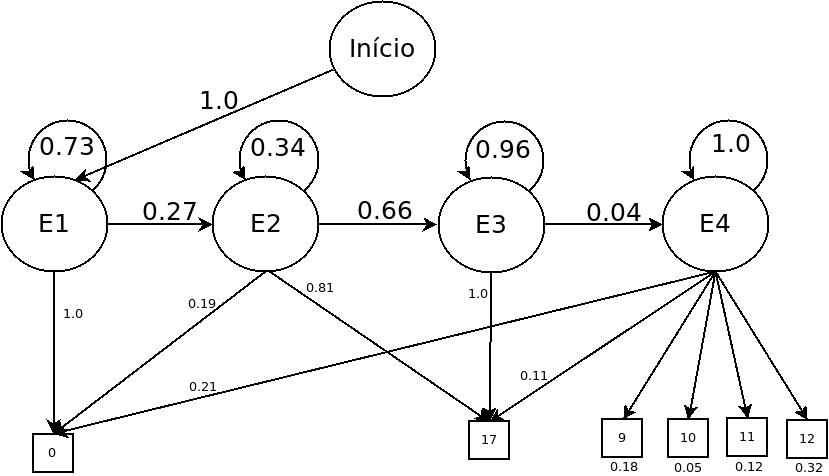
\includegraphics[scale=0.35]{imagens/HMM_3_apos_treino.jpg}
  \label{img:HMM_3_apos_treino}
\end{figure}

\begin{figure}[!htbp]
  \center
  \caption{Parâmetros de uma HMM treinada com os vídeos de passos a direita.}
  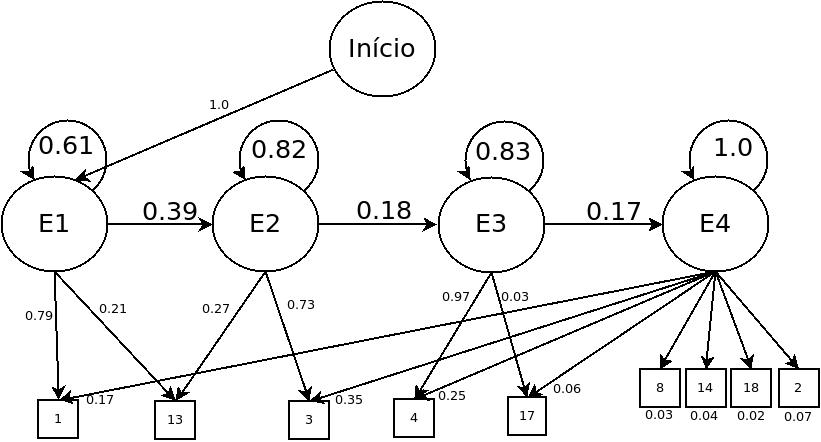
\includegraphics[scale=0.35]{imagens/HMM_1_apos_treino.jpg}
  \label{img:HMM_1_apos_treino}
\end{figure}

\begin{figure}[!htbp]
  \center
  \caption{Parâmetros de uma HMM treinada com os vídeos de passos a esquerda.}
  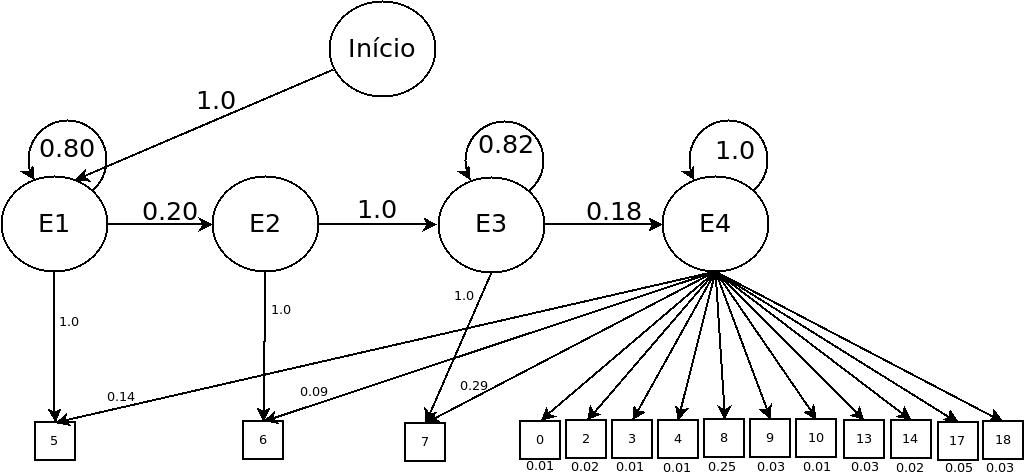
\includegraphics[scale=0.35]{imagens/HMM_2_apos_treino.jpg}
  \label{img:HMM_2_apos_treino}
\end{figure}


\subsection{Modelo de identificação}

A cada segundo de vídeo os últimos trinta símbolos são armazenados em um vetor e avaliados pelo algoritmo de Viterbi em cada uma das cinco HMMs, o retorno é a sequência do caminho mais provável e a probabilidade desse caminho em cada um dos cinco modelos respectivamente. Um outro vetor armazena todas essas probabilidades para avaliação posterior da maior delas e consequentemente o gesto mais provável. Depois dessa avaliação o vetor de símbolos é esvaziado para ser preenchido novamente no próximo segundo.

Na maioria dos reconhecimentos, a sequência recebida só retornava probabilidade em uma das HMMs, todas as outras tinham chance nula de ser a HMM responsável pela sequência de símbolos de entrada. Para ilustrar essa situação, observe um exemplo de vetor de símbolos que foi armazenado em um dos segundo de uma sequência de vídeo onde o usuário está caminhando para a direita, que gerou a seguinte sequência de símbolos observáveis: \[[1, 1, 1, 1, 2, 3, 3, 3, 3, 3, 8, 4, 4, 4, 4, 4, 17, 17, 1, 1, 1, 2, 3, 3, 3, 3, 8, 4, 4, 4].\] A Tabela \ref{table:viterbi_1} exibe as probabilidades calculadas através dos caminhos mais prováveis, em todas as HMMs, dessa sequência de símbolos acontecer.

Se observarmos os grafos das HMMs treinadas, verificaremos que a probabilidade é nula na segunda HMM, porque ela tem não tem chance alguma de retornar o símbolo 1, enquanto a terceira, quarta e quinta também tem probabilidade nula de retornar os símbolos 2, 3 e 4.

Quando a todos os modelos retornam probabilidade nula, nenhum gesto é reconhecido naquele segundo e nenhum comando é enviado ao avatar no ambiente virtual, portanto ele fica executando uma animação default, enquanto aguarda um reconhecimento bem sucedido.

\begin{table}[!htbp]
\caption{Tabela de exemplo de probabilidades avaliadas pelo algoritmo de Viterbi.}
\label{table:viterbi_1}
\centering
\begin{tabular}{p{5.5cm} | p{5.5cm}}
\toprule
\textbf{HMM} & \textbf{Probabilidade} \\
\midrule[1pt]
1 - Passo para direita & -63.091143841560843 \\ \midrule
2 - Passo para esquerda & Nenhuma \\ \midrule
3 - Levantar braço direito & Nenhuma \\ \midrule
4 - Levantar braço esquerdo & Nenhuma \\ \midrule
5 - Levantar ambos os braços & Nenhuma \\
\bottomrule
\end{tabular}
\end{table}


  \Chapter{Interação com o avatar}

 Nessa etapa, para construção do ambiente virtual, o software Blender\footnote{Blender - http://www.blender.org/} foi utilizado para modelagem, e para a produção das animações do avatar. A biblioteca PyGame\footnote{PyGame - http://www.pygame.org} foi usada como motor gráfico (engine).

Blender é um software multiplataforma de modelagem, animação, texturização, composição, renderização,
edição de vídeo e criação de aplicações interativas em 3D, como jogos, através de seu
motor de jogo integrado, o Blender Game Engine, inclui suporte a Python como linguagem
script, que pode ser usada tanto no Blender quanto em seu motor de jogo, e possui código aberto.
Ele está sob a licença GNU-GPL, que permite a qualquer pessoa ter acesso ao código-fonte do programa \cite{Blender3D}.

PyGame é um conjunto de módulos em Python projetado para jogos. Permitindo que games e programas de multimidia completos sejam escritos na linguagem Python. É gratuito, portátil, código aberto, não requer OpenGL\footnote{OpenGL (Open Graphics Library) - http://www.opengl.org/} e usa funções otimizadas em C e Assembly para funções essenciais.

Na Figura \ref{img:ambiente_virtual} o avatar (agente que representa o usuário) está no ambiente virtual executando a animação de estado de espera (\textit{default}) enquanto nenhum gesto é reconhecido. O ambiente virtual é definido pela imagem de fundo, pelo avatar e outros objetos que possam futuramente ser inseridos no cenário.

\begin{figure}[!htbp]
  \center
  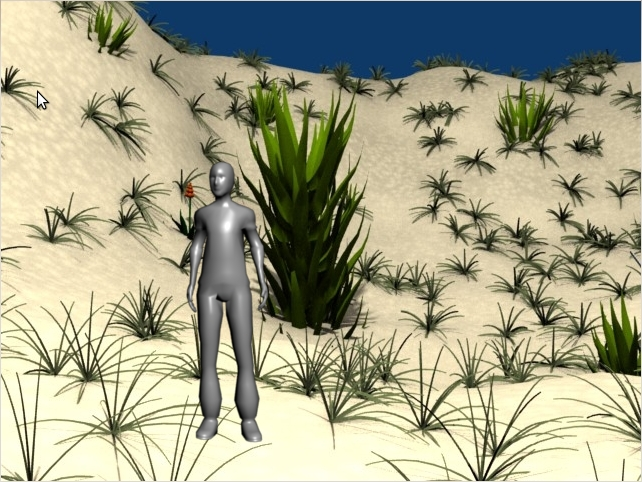
\includegraphics[scale=0.40]{imagens/ambiente_virtual.jpg}
  \caption{Ambiente Virtual.}
  \label{img:ambiente_virtual}
\end{figure}


\section{Criando as animações}

Existem sites que são repositórios online de diversos modelos em 3D, como pessoas, carros, roupas, etc, disponíveis em diferentes formatos de acordo com os vários softwares de modelagem 3D. Blender também possui esses repositórios online, o avatar usado nesse sistema foi baixado de um repositório online gratuito.

Para produzir as animações, é preciso salvar as diferentes poses desses modelos no decorrer dos frames. Nesse sistema a taxa de quadros é trinta, então com a finalidade de evitar incoerências, as animações do avatar também foram gravadas a uma taxa de trinta quadros por segundo.

Os modelos são ligados a um tipo de esqueleto, chamado de \textit{armature}, que dita quais são as articulações do modelo. As rotações e translações das partes do modelos são feitas de acordo com a quantidade e local dos membros do esqueleto. A Figura \ref{img:armature} exibe a posição desse esqueleto nos quadros 1, 15 e 30. Blender automaticamente produz os frames intermediários entre essas poses. Os frames são exportados em imagens no formato PNG\footnote{PNG - Portable Network Graphics}, porque esse formato suporta o canal alfa e isso permite que o fundo possa ser retirado e substituído pelo fundo escolhido para o ambiente virtual.

\begin{figure}[!htbp]
  \centering
  \subfigure[Frame 1]{\includegraphics[width=4cm]{imagens/armature_1.jpg}}
  \subfigure[Frame 15]{\includegraphics[width=4cm]{imagens/armature_15.jpg}}
  \subfigure[Frame 30]{\includegraphics[width=4cm]{imagens/armature_1.jpg}}
  \caption{Posição da armature em frames selecionados.}
  \label{img:armature}
\end{figure}

\section{Criando as interações}

As sequências das animações exportadas pelo Blender são armazenadas para serem utilizadas em tempo real pelo motor gráfico, em nosso sistema o PyGame. As imagens são armazenadas em vetores e a todo momento uma função atualiza na tela a impressão do fundo e do avatar.

Para as animações onde o avatar caminha para a esquerda ou direita, sua posição no ambiente também é alterada, subtraindo-se e adicionando da variável que armazena sua localização no eixo X.

Toda vez que um gesto é reconhecido pelo módulo de identificação, esse gesto é armazenado em uma fila, responsável pela sequência das animações. Ao final de cada animação, o primeiro elemento da fila é retirado dela e executado pelo avatar. Uma variável responsável pelo estado do avatar recebe os valores dessa fila em ordem. Essa estrutura foi utilizada para evitar que a animação atual do avatar fosse interrompida bruscamente caso um gesto novo fosse identificado antes desse animação ter sido concluída.

A Figura \ref{img:animacoes} mostra alguns frames das animações utilizadas para cada um dos gestos no sistema, inclusive a animação executada enquanto nenhum gesto é identificado (default) e a Figura \ref{img:fundo_ambiente_virtual} a imagem de fundo do ambiente virtual, que pode ser substituída por qualquer outra imagem.

\begin{figure}[!htbp]
  \center
  \includegraphics[scale=0.25]{imagens/fundo_ambiente_virtual.jpg}
  \caption{Fundo do Ambiente Virtual.}
  \label{img:fundo_ambiente_virtual}
\end{figure}


\begin{figure}[!htbp]
\center
\begin{tabular}{ccccccc}
\subfigure{\includegraphics[scale=0.25]{imagens/standing_animation_1.jpg}} & \hspace{0.5cm} &
\subfigure{\includegraphics[scale=0.25]{imagens/standing_animation_2.jpg}} & \hspace{0.5cm} &
\subfigure{\includegraphics[scale=0.25]{imagens/standing_animation_3.jpg}} & \hspace{0.5cm} &
\subfigure{\includegraphics[scale=0.25]{imagens/standing_animation_4.jpg}}
\\

\subfigure{\includegraphics[scale=0.25]{imagens/walk_left_animation_1.jpg}} & &
\subfigure{\includegraphics[scale=0.25]{imagens/walk_left_animation_2.jpg}} & &
\subfigure{\includegraphics[scale=0.25]{imagens/walk_left_animation_3.jpg}} & &
\subfigure{\includegraphics[scale=0.25]{imagens/walk_left_animation_4.jpg}}
\\
\subfigure{\includegraphics[scale=0.25]{imagens/walk_right_animation_1.jpg}} & &
\subfigure{\includegraphics[scale=0.25]{imagens/walk_right_animation_2.jpg}} & &
\subfigure{\includegraphics[scale=0.25]{imagens/walk_right_animation_3.jpg}} & &
\subfigure{\includegraphics[scale=0.25]{imagens/walk_right_animation_4.jpg}}
\\
\subfigure{\includegraphics[scale=0.25]{imagens/right_arm_up_animation_1.jpg}} & &
\subfigure{\includegraphics[scale=0.25]{imagens/right_arm_up_animation_2.jpg}} & &
\subfigure{\includegraphics[scale=0.25]{imagens/right_arm_up_animation_3.jpg}} & &
\subfigure{\includegraphics[scale=0.25]{imagens/right_arm_up_animation_4.jpg}}
\\
\subfigure{\includegraphics[scale=0.25]{imagens/left_arm_up_animation_1.jpg}} & &
\subfigure{\includegraphics[scale=0.25]{imagens/left_arm_up_animation_2.jpg}} & &
\subfigure{\includegraphics[scale=0.25]{imagens/left_arm_up_animation_3.jpg}} & &
\subfigure{\includegraphics[scale=0.25]{imagens/left_arm_up_animation_4.jpg}}
\\
\subfigure{\includegraphics[scale=0.25]{imagens/both_arms_up_animation_1.jpg}} & &
\subfigure{\includegraphics[scale=0.25]{imagens/both_arms_up_animation_2.jpg}} & &
\subfigure{\includegraphics[scale=0.25]{imagens/both_arms_up_animation_3.jpg}} & &
\subfigure{\includegraphics[scale=0.25]{imagens/both_arms_up_animation_4.jpg}}
\end{tabular}
\caption{Frames 1, 5, 10 e 15 das animações criadas para o avatar.}
\label{img:animacoes}
\end{figure}


  \Chapter{Resultados e discussões}

Um sistema, cujo objetivo principal era implementar um forma de interação homem-máquina de forma não convencional através de reconhecimento de gestos por visão computacional, foi implementado neste trabalho. O modelo é testado utilizando-se cinco vídeos gravados de cada um dos gestos isolados, outros vídeos foram gravados onde os mesmos gestos apresentavam-se de forma contínua e por último um vídeo longo onde todos os gestos são realizados intercalados de forma contínua sem ordem prevista. Um vídeo de outro usuário executando os gestos também foi gravado com a finalidade de testar os resultados do aplicativo.

Como visto anteriormente, um avatar foi desenvolvido para que técnicas de visão computacional pudessem ser utilizadas em conjunto com modelos ocultos de Markov com o objetivo de enviar comandos de controle para esse avatar atuar no ambiente virtual.


\section{A aplicação em interação com objetos virtuais}

Os módulos de vídeos e ambiente virtual são inicializados ao mesmo tempo, então a captura de cada frame do vídeo é iniciada. O avatar fica realizando a animação padrão, enquanto o módulo de identificação reconhece o gesto realizado no último segundo.

As Figuras \ref{img:sistema_1}, \ref{img:sistema_2}, \ref{img:sistema_3} e \ref{img:sistema_4} exibem imagens do sistema reconhecendo os gestos corretamente e o avatar realizando as animações equivalentes. A Figura \ref{img:sistema_krishynan} demonstra um outro usuário utilizando o sistema, mas não tendo participado do processo de treinamento, ou seja, um usuário B utilizou o mesmo módulo de treino que foi alimentado com vídeos do usuário A.

\begin{figure}[!htbp]
  \includegraphics[scale=0.35]{imagens/sistema_1.jpg}
  \caption{Situação de reconhecimento do gesto levantar o braço esquerdo no sistema.}
  \label{img:sistema_1}
\end{figure}

\begin{figure}[!htbp]
  \includegraphics[scale=0.35]{imagens/sistema_2.jpg}
  \caption{Situação de reconhecimento do gesto passo para esquerda no sistema.}
  \label{img:sistema_2}
\end{figure}

\begin{figure}[!htbp]
  \includegraphics[scale=0.35]{imagens/sistema_3.jpg}
  \caption{Situação de reconhecimento do gesto passo para direita no sistema.}
  \label{img:sistema_3}
\end{figure}

\begin{figure}[!htbp]
  \includegraphics[scale=0.35]{imagens/sistema_4.jpg}
  \caption{Outra situação de reconhecimento do gesto levantar o braço esquerdo no sistema.}
  \label{img:sistema_4}
\end{figure}

\begin{figure}[!htbp]
  \includegraphics[scale=0.35]{imagens/sistema_krishynan.jpg}
  \caption{Usuário B testando o sistema treinado pelo usuário A.}
  \label{img:sistema_krishynan}
\end{figure}

O sistema não se comportou de forma esperada quando um gesto de andar para direita ou para esquerda acontecia seguido da postura parado de frente para a câmera. Isso aconteceu principalmente porque os vídeos que treinaram o sistema não continham um exemplo desse gesto, em outras palavras, as HMMs treinadas para reconhecerem os gestos de passos, nunca começavam com o símbolo 0, que é a codeword para a postura parado de frente, então o gesto de caminhar só era reconhecido se o usuário já estivesse de lado no ínicio das sequências desses gestos. A Figura \ref{img:andar_from_parado} ilustra o gesto acima descrito.

\begin{figure}[!htbp]
  \centering
  \subfigure{\includegraphics[scale=0.35]{imagens/andar_from_parado_1.jpg}}
  \subfigure{\includegraphics[scale=0.35]{imagens/andar_from_parado_2.jpg}}
  \subfigure{\includegraphics[scale=0.35]{imagens/andar_from_parado_3.jpg}}
  \subfigure{\includegraphics[scale=0.36]{imagens/andar_from_parado_4.jpg}}
  \caption{Gesto não reconhecido nos primeiros testes do sistema.}
  \label{img:andar_from_parado}
\end{figure}


Essa situação foi resolvida, injetando alguns símbolos 0 nas sequências de treinos dessas HMMs. As Figuras \ref{img:HMM_1_apos_treino_2} e \ref{img:HMM_2_apos_treino_2} apresentam os grafos dessas novas HMMs.

\begin{figure}[!htbp]
  \center
  \includegraphics[scale=0.35]{imagens/HMM_1_apos_treino_2.jpg}
  \caption{Parâmetros da HMM treinada com os vídeos do gesto passo para direita após a injeção de símbolos 0.}
  \label{img:HMM_1_apos_treino_2}
\end{figure}

\begin{figure}[!htbp]
  \center
  \includegraphics[scale=0.35]{imagens/HMM_2_apos_treino_2.jpg}
  \caption{Parâmetros da HMM treinada com os vídeos do gesto passo para esquerda após a injeção de símbolos 0.}
  \label{img:HMM_2_apos_treino_2}
\end{figure}

Essas HMMs reconhecem com sucesso os gestos anteriormente descritos, porém os gestos que eram reconhecidos antes agora não são reconhecidos, porque essas HMM só reconhecem os gestos de caminhar se as sequências forem inicializadas com o símbolo 0.

Esse problema foi resolvido alterando no processo de modelagem dessas duas HMMs, os parâmetros do vetor \(\pi\), que passaram a assumir valores com probabilidades iguais de começar em qualquer um dos quatro estados
\[
 \pi =
 \begin{pmatrix}
  0.25 & 0.25 & 0.25 & 0.25
 \end{pmatrix}.
\]

A topologia dessas HMM também foi alterada para o modelo totalmente conectado, isso resolveu o problema de forma que o gesto, além de poder começar em qualquer um dos estados, todos os estados poderiam retornar as quatro codewords de seus gestos. Agora o gesto de andar para direita, por exemplo, poderia começar pelas codewords 0, 1, 2, 3 ou 4 e todas esses símbolos poderiam aparecer em qualquer ordem que a sequência ainda seria reconhecida.

Se o interesse fosse manter a topologia \textit{Left Right Banded}, devido a sua taxa melhor de detecção segundo os trabalhos anteriormente comentados, seria preciso criar duas HMMs para cada gesto de caminhar.
 Um para a situação onde o usuário já se encontra de lado e outra para a situação onde o usuário se encontra virado de frente para a câmera. Essa situação também poderia ser resolvida, fazendo-se pequenas alterações na HMM treinada para que no seu primeiro estado ela possa retornar tanto o símbolo 1 quanto o símbolo 0. Avaliar se essas soluções apresentarão melhores probabilidades nos reconhecimentos é um dos motivos para trabalhos futuros.

Outro problema encontrado é quando o usuário fica parado em frente a câmera sem executar gesto algum, haverá uma sequência contendo apenas símbolos 0 nesse caso, se um pequeno ruído entrar nessa sequência, por exemplo, um simbolo de algum gesto de levantar o braço, uma das HMM vai retornar uma probabilidade mesmo que muito baixa, daquele gesto ter acontecido e ele na verdade não aconteceu. Seria preciso criar uma HMM para a situação do usuário ficar parado na maior parte do tempo ou definir uma tolerância nas probabilidades, para que quando uma probabilidade for muito baixa esse gesto não seja enviado para o módulo do ambiente virtual. Avaliar essas soluções e decidir qual seria melhor, também é motivo para trabalhos futuros.

Mesmo considerando esses problemas, o desempenho do sistema é muito satisfatório.



  \Chapter{Conclusões e trabalhos futuros}

Neste trabalho foi implementado um avatar em um ambiente virtual que recebe comandos do usuário através de visão computacional e técnicas de reconhecimento de padrões. O sistema baseou-se em algoritmos de segmentação no processo de captura e extração da silhueta do usuário a partir de um câmera. É importante ter um ambiente onde exista luz controlada, evitando-se assim variações na iluminação e muitos ruídos no sinal da silhueta extraída.

Vinte e uma posturas foram definidas, quatro para cada um dos cinco gestos definidos e uma para a situação onde o usuário está parado. Os gestos são: Caminhar para a direita, caminhar pra esquerda, levantar o braço direito, levantar o braço esquerdo e levantar ambos os braços.

Para extração das características das imagens foi utilizado uma malha que contabilizou a relação de pixels brancos em cada um de seus segmentos na silhueta. O classificador utilizado para as postura foi quantização vetorial. Vinte e uma imagens foram escolhidas para representar os centros de seus grupos e as imagens passaram a ser descritas com o índice do centro do grupo ao qual elas foram agrupadas.

Uma sequência de posturas descreve um gesto, o classificador utilizado para essas sequências foi cadeia oculta de Markov, uma foi criada para cada gesto, contendo cada uma quatro estados, de acordo com a quantidade de posturas para cada gestos.

Esses modelos foram treinadas com o algoritmo de Baum-Welch e tendo como entrada sequências de quatro diferentes vídeos para cada gestos, do respectivo gesto sendo executado de forma isolada.

A todo segundo uma sequência de trinta símbolos é enviada para o algoritmo de Viterbi analisar a probabilidade dessa sequência ocorrer em cada uma das cinco HMMs e a que retornar maior probabilidade envia um comando correspondente para o ambiente virtual.

O ambiente virtual é composto de um avatar que fica aguardando comandos de entrada que decidirão qual animação será executada, esses gestos são guardados em uma fila no momento em que são detectados e saem da fila a toda vez que o avatar conclui uma animação.

Esse sistema atendeu aos objetivos desse trabalho, que era desenvolver um modelo de reconhecimento de gestos a partir de visão computacional, promovendo assim um meio de interação homem/máquina mais natural do que os convencionais mouse e teclado.


\section{Trabalhos futuros}

Novas possibilidades de desenvolvimento de outras formas de interação homem/máquina baseados em visão computacional são estimuladas a partir do sistema proposto nesse trabalho. Partes deste modelo podem ser utilizadas na criação de outros sistemas ou a partir dele, como os modelos de segmentação, quantização ou os modelos de Markov ocultos implementados.

Segue abaixo, algumas atividades que poderiam acontecer para evoluir o sistema implementado, a partir do sistema atual.

\begin{itemize}

\item Estudar a possibilidade de se usar o acessório Kinect em conjunto com HMMs para análise das sequências de sinais.

\item Implementar um algoritmo de subtração de fundo mais robusto, que possa lidar com problemas relacionados a iluminação e fundos mais complexos.

\item Criar e treinar novas HMMs para reconhecerem mais gestos e mais comandos possam ser enviados ao ambiente virtual.

\item Expandir o numéro de animações do avatar e criar outros objetos com os quais ele poderia interagir no cenário.

\item Avaliar a possibilidade de utilização de outras características para criação do vetor de características ou expandi-lo, o objetivo é garantir uma maior taxa de acertos das posturas.

\end{itemize}



  \anexo


  %--------------------------------- Bibliografia ------------------------------

  \citeoption{abnt-repeated-author-omit=yes}
  \bibliographystyle{abnt-alf}
  \bibliography{bibliografia}
\end{document}

